\chapter{Результаты} \label{chapt_Res}

\section{Инвариантные спектры по поперечному импульсу} \label{sectRes_spectra}

Инвариантные спектры по поперечному импульсу были вычислены согласно формуле \ref{eq:spectra}.
\begin{equation}
	\label{eq:spectra}
	\frac{1}{2\pi p_T} \frac{d^2 N}{dp_T dy}=\frac{1}{2\pi p_T}\frac{N_h}{N_{evt} \varepsilon_{eff} \Delta p_T \Delta y}
\end{equation}
где $\Delta p_T$ – диапазон поперечных импульсов;

$\Delta y$ – диапазон быстрот;

$N_h$ - количество заряженных адронов $h$, зарегистрированных в диапазонах  $\Delta p_T, \Delta y$;

\eff~ -- эффективность регистрации адронов $h$. 

Для оценки значения величины \eff~ было проведено Монте-Карло моделирование (см. гл. \ref{sect3:EffRec}).
Инвариантные спектры по поперечному импульсу, измеренные для положительно и отрицательно заряженных адронов в различных центральностях $p$+Al, \heau, Cu+Au и U+U столкновений представлены на рис. \ref{img:SpectraPt0}, \ref{img:SpectraPt1}. 

\begin{figure}[] 
	\centerfloat
	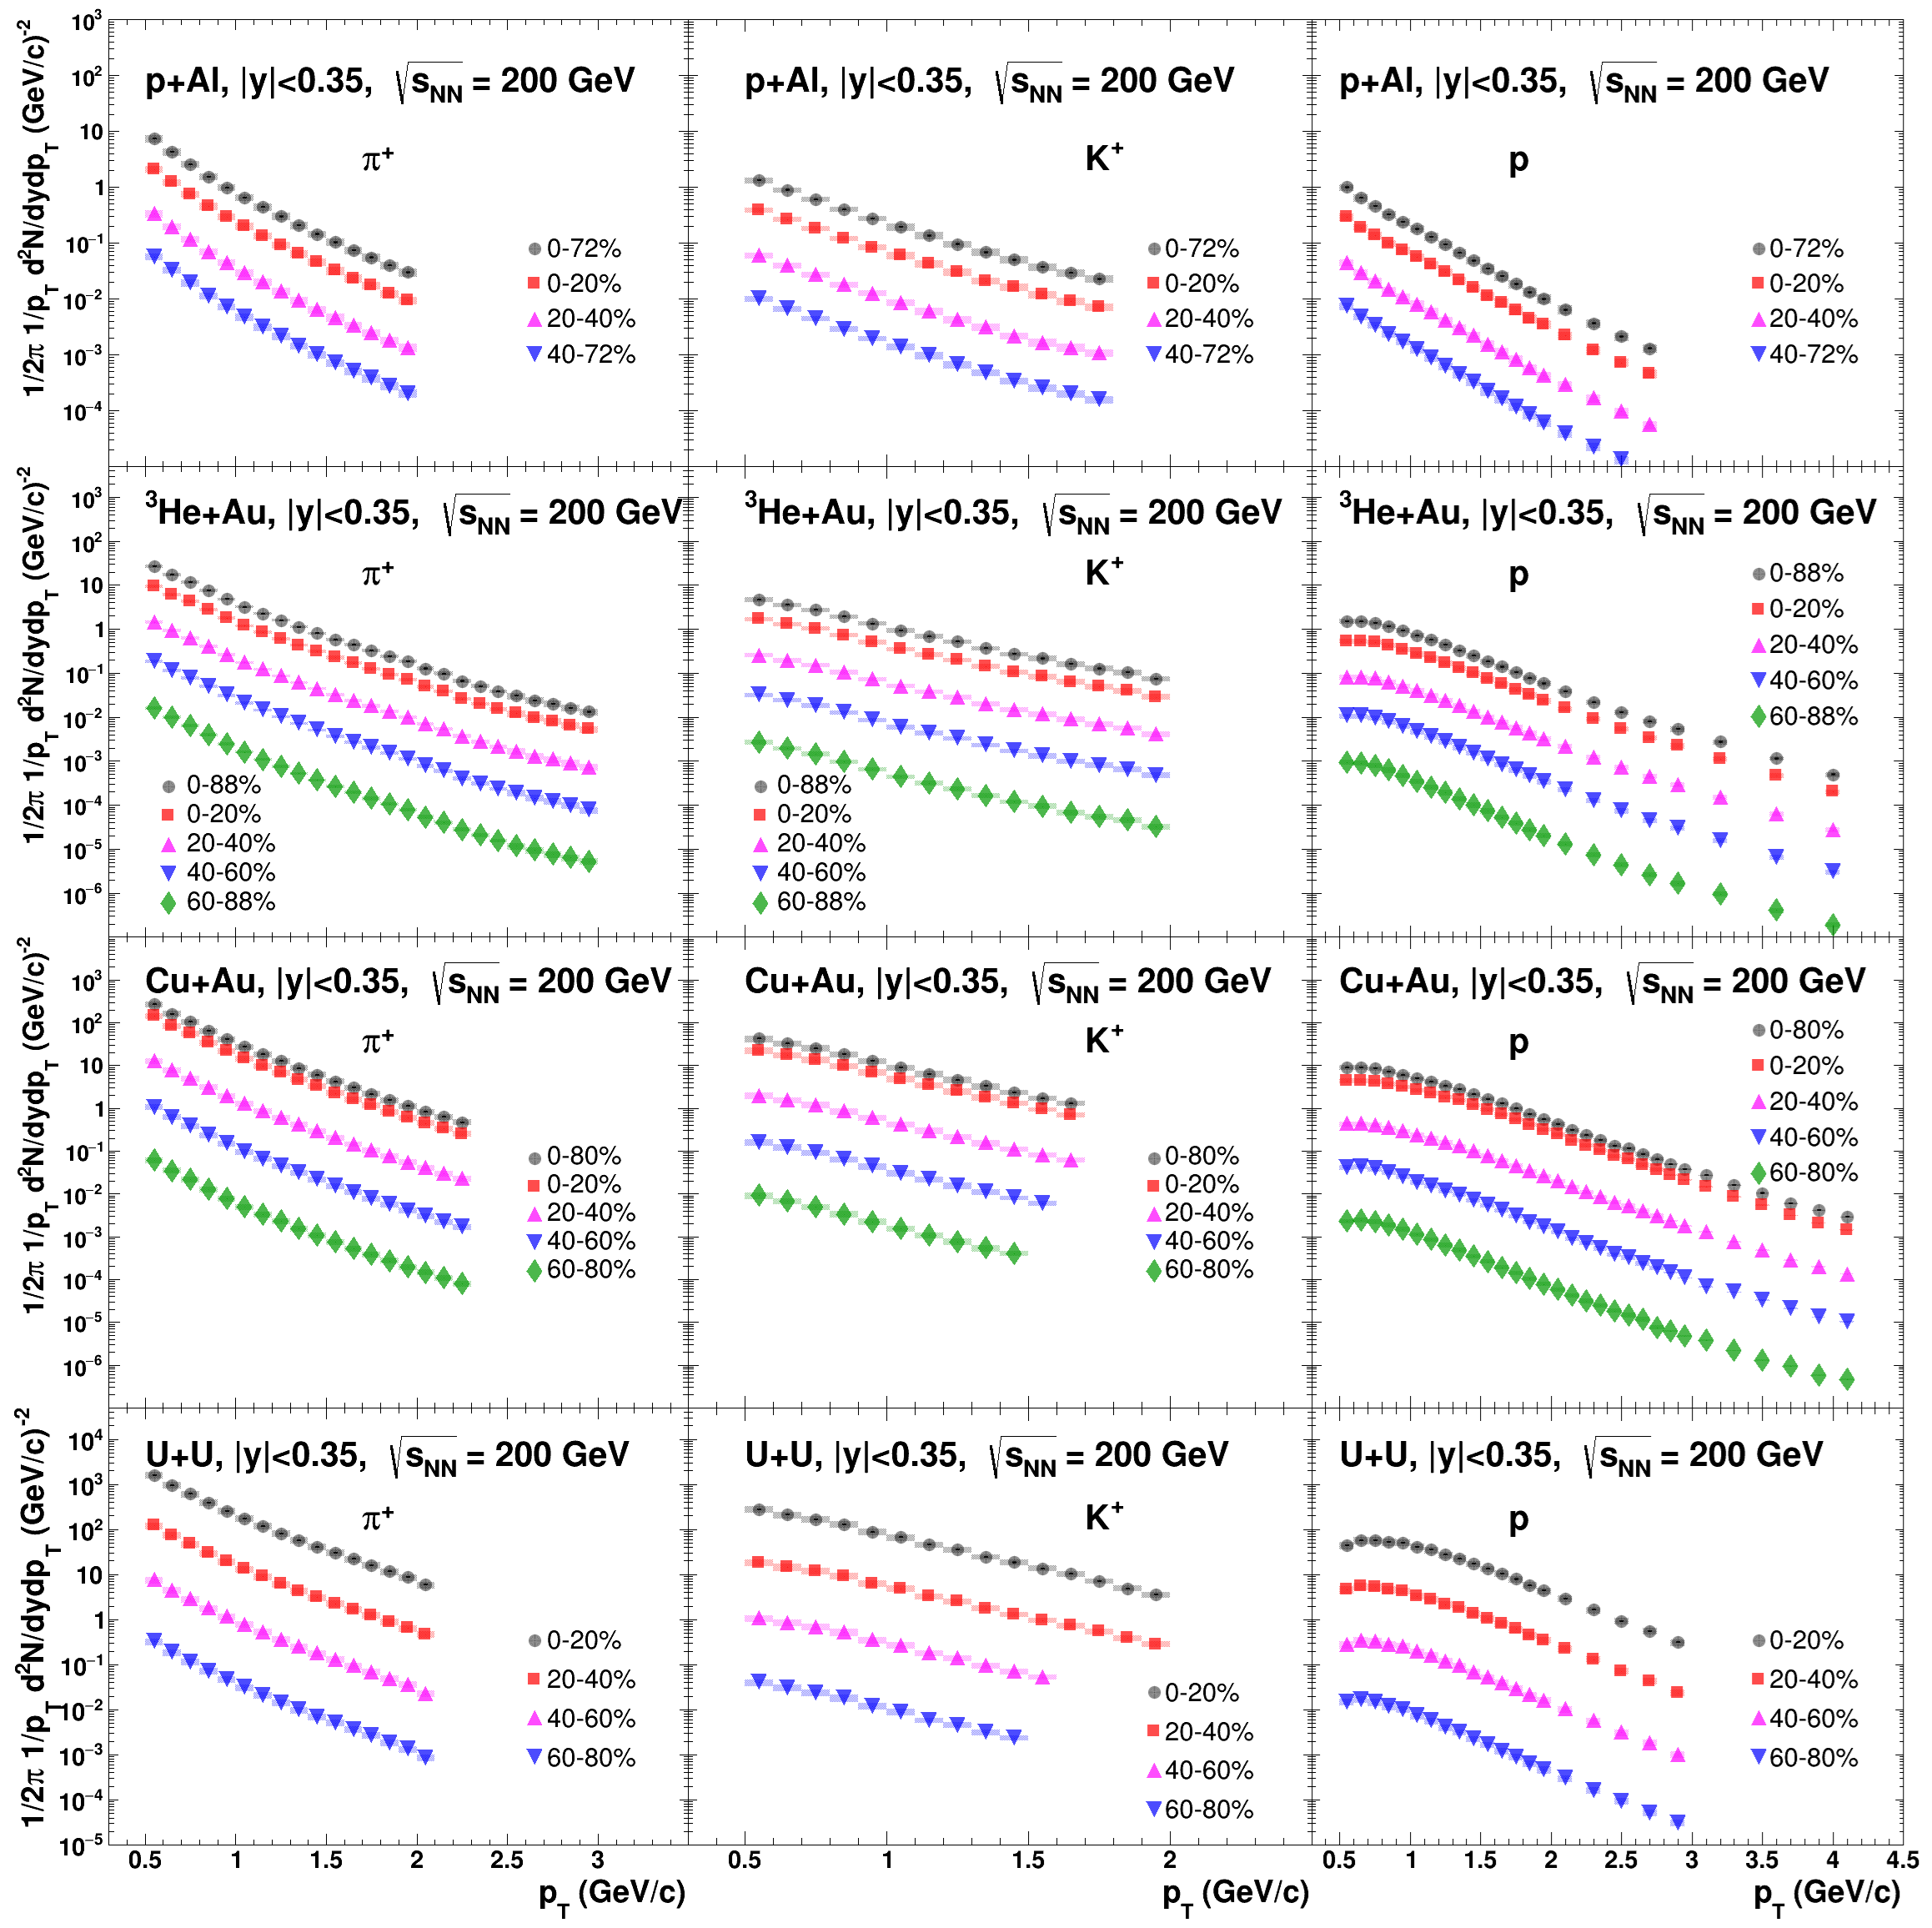
\includegraphics [width=1\linewidth]{Results/spectraDiss_pt_0.png}
	\caption{Инвариантные спектры по поперечному импульсу, измеренные для $\pi^+$, $K^+$, $p$ в различных центральностях p+Al, \heau, Cu+Au и U+U столкновениях.} 
	\label{img:SpectraPt0}
\end{figure}
\begin{figure}[] 
	\centerfloat
	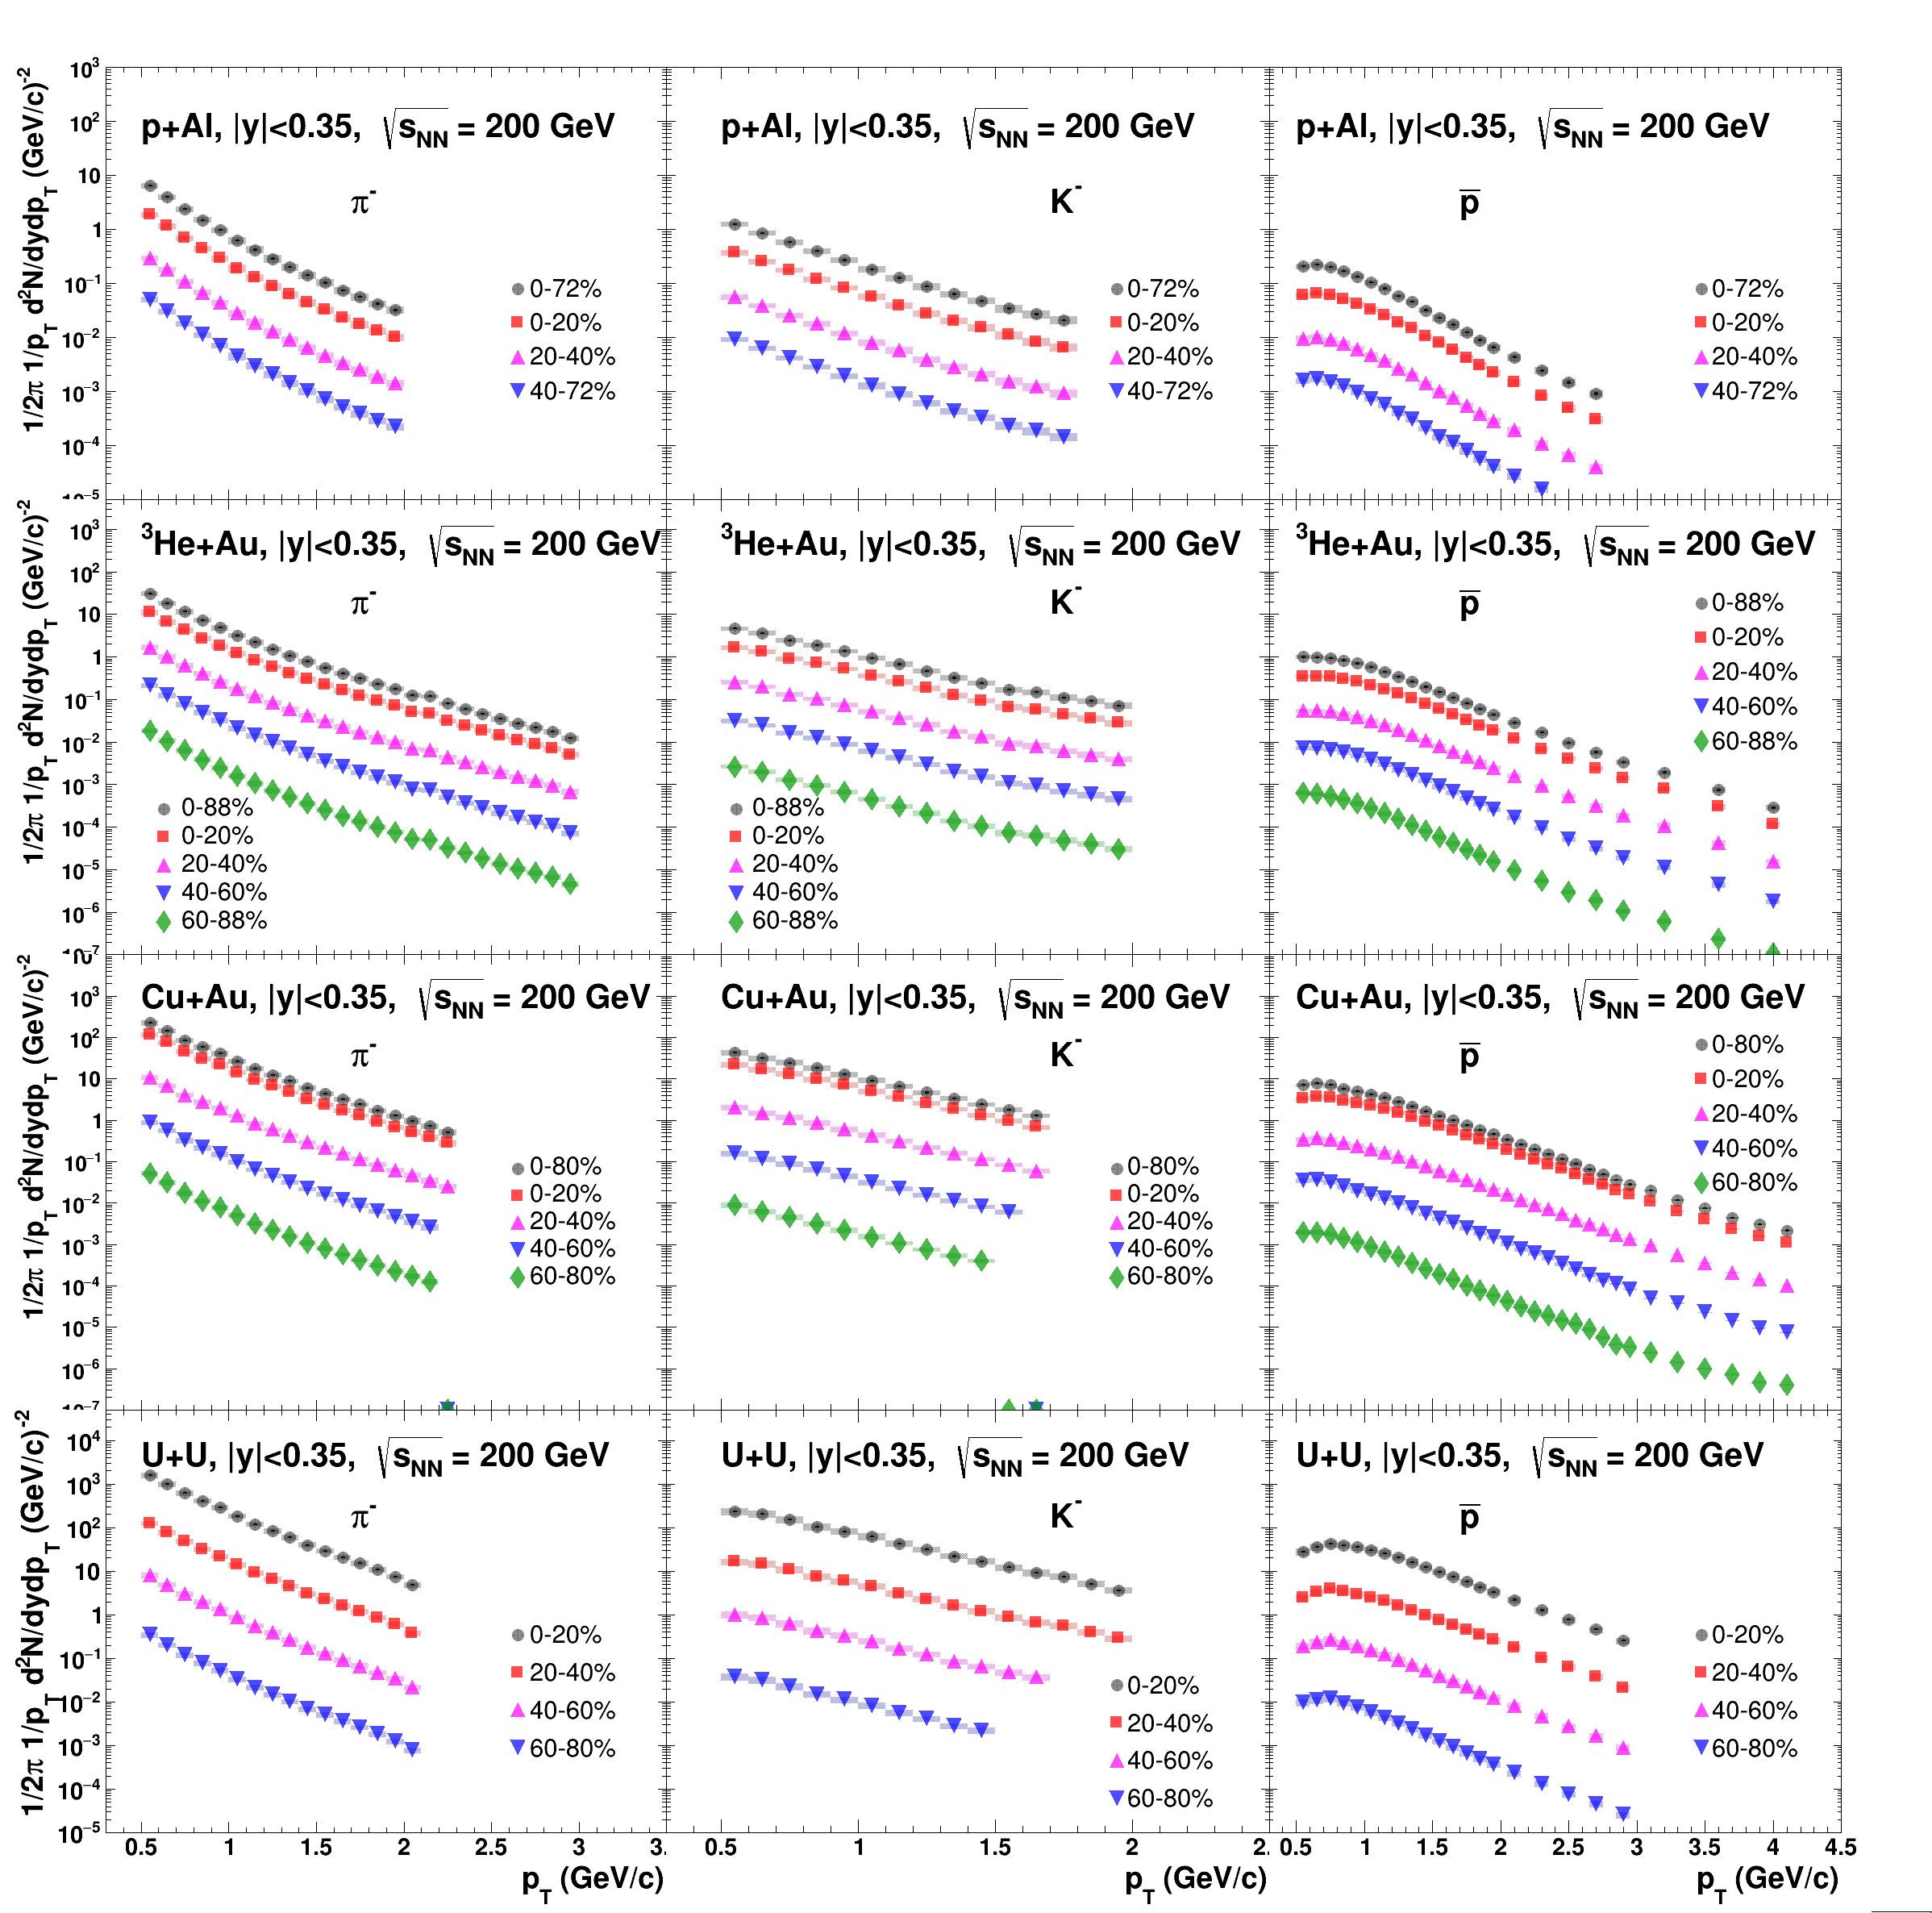
\includegraphics [width=1\linewidth]{Results/spectraDiss_pt_1.png}
	\caption{Инвариантные спектры по поперечному импульсу, измеренные для $\pi^-$, $K^-$, $\bar{p}$ в различных центральностях p+Al, \heau, Cu+Au и U+U столкновениях.} 
	\label{img:SpectraPt1}
\end{figure}



\section{Факторы ядерной модификации} \label{sectRes_rab}


\begin{figure}[] 
	\centerfloat
	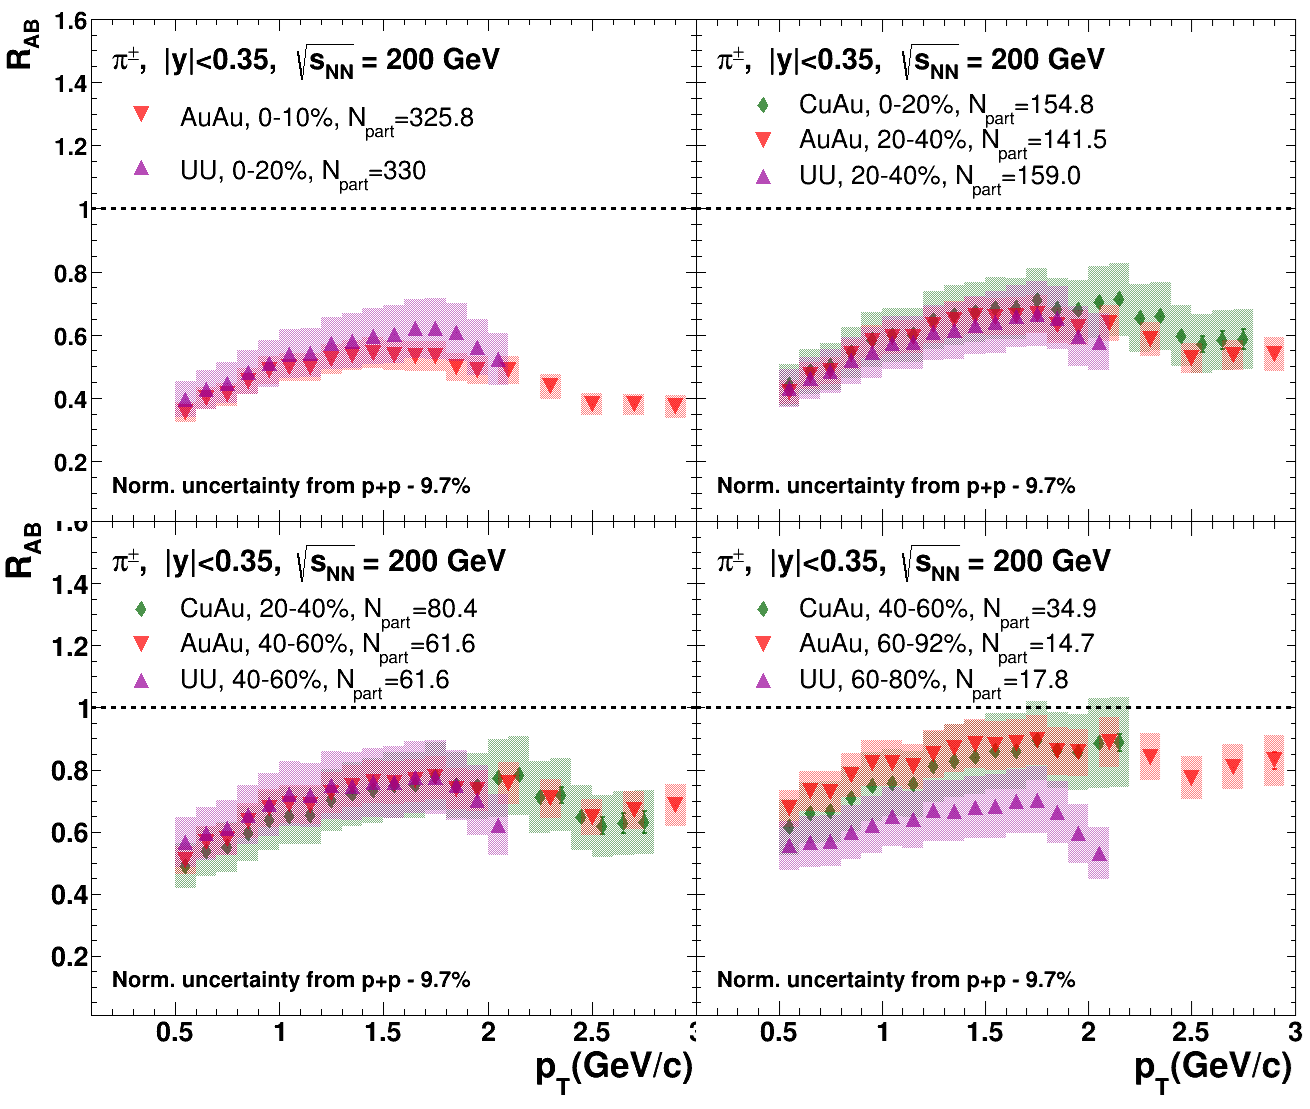
\includegraphics [width=0.7\linewidth]{Results/DrawAll_large_raa_1}
	\caption{Значения \rab \ измеренные для \pipm \ в различных центральностях \cuau, \auau, \uu \ столкновений.} 
	\label{img:Res_piRab_large}
\end{figure}

\begin{figure}[] 
	\centerfloat
	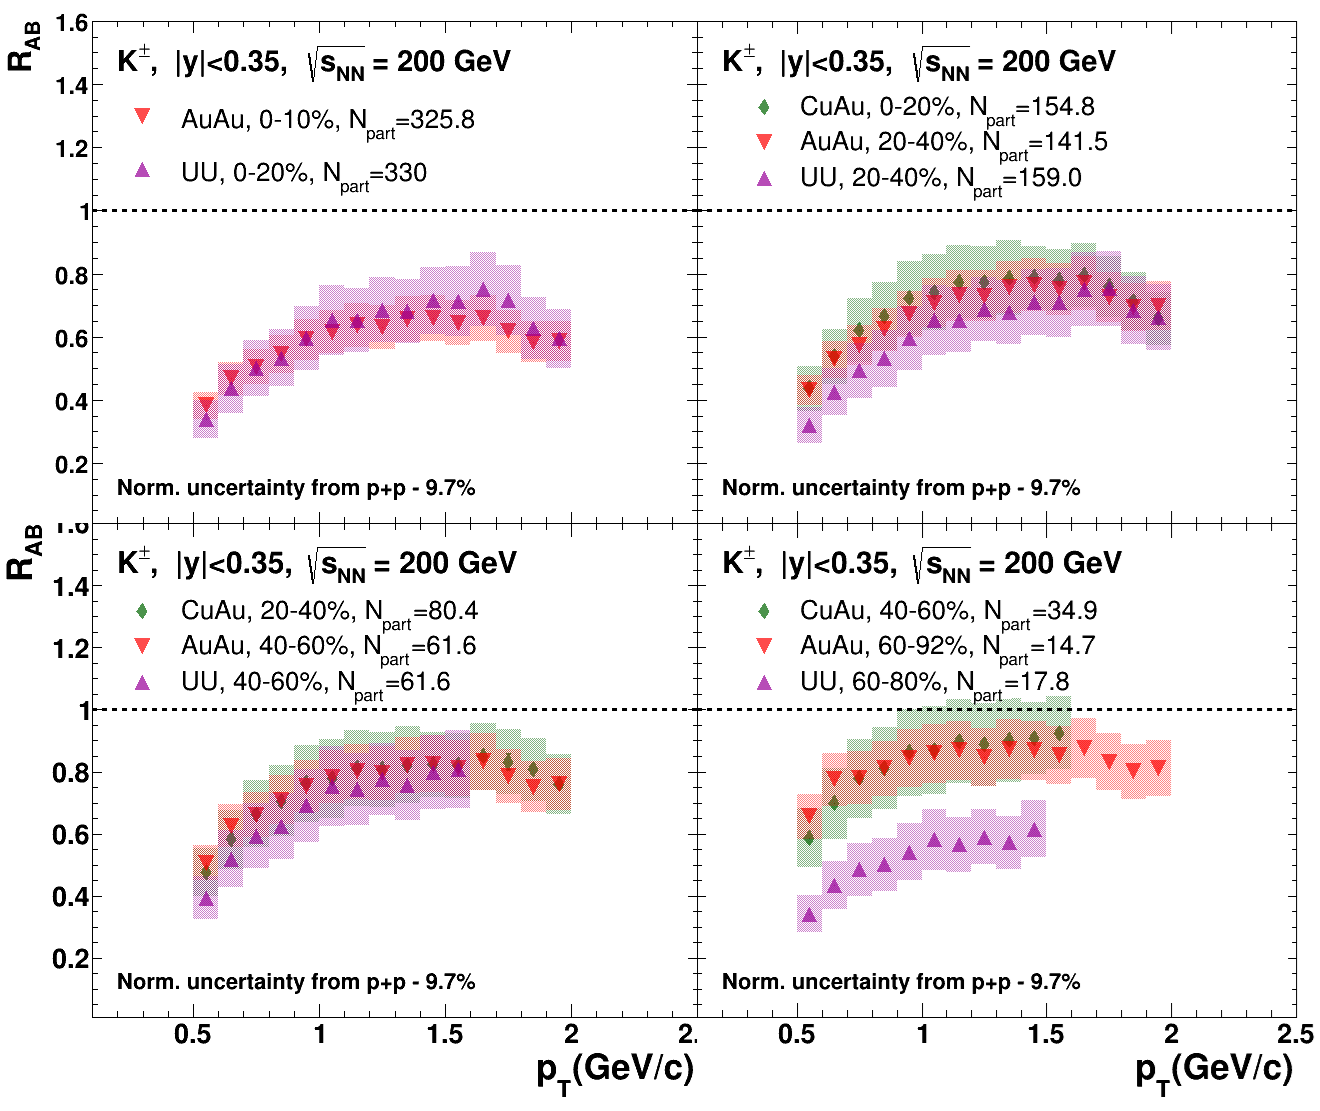
\includegraphics[width=0.7\linewidth]{Results/DrawAll_large_raa_2}
	\caption{Значения \rab \ измеренные для \Kpm \ в различных центральностях \cuau, \auau, \uu \ столкновений.} 
	\label{img:Res_KRab_large}
\end{figure}

\begin{figure}[] 
	\centerfloat
	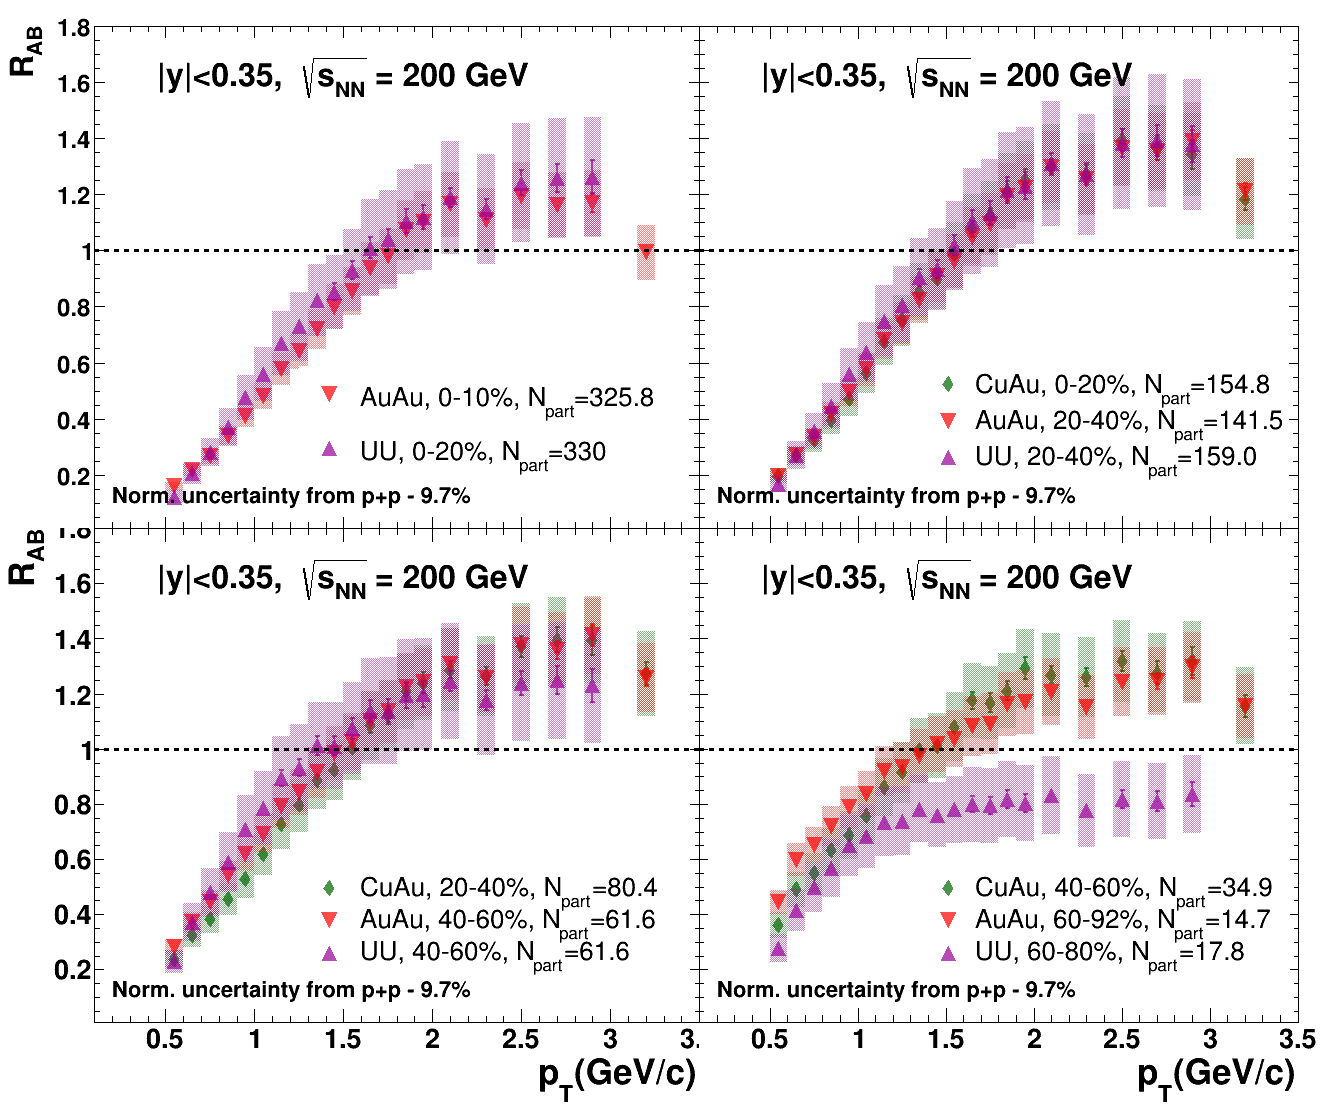
\includegraphics[width=0.7\linewidth]{Results/DrawAll_large_raa_3}
	\caption{Значения \rab измеренные для \prots \ в различных центральностях \cuau, \auau, \uu \ столковений.} 
	\label{img:Res_pRab_large}
\end{figure}

\begin{figure}[] 
	\centerfloat
	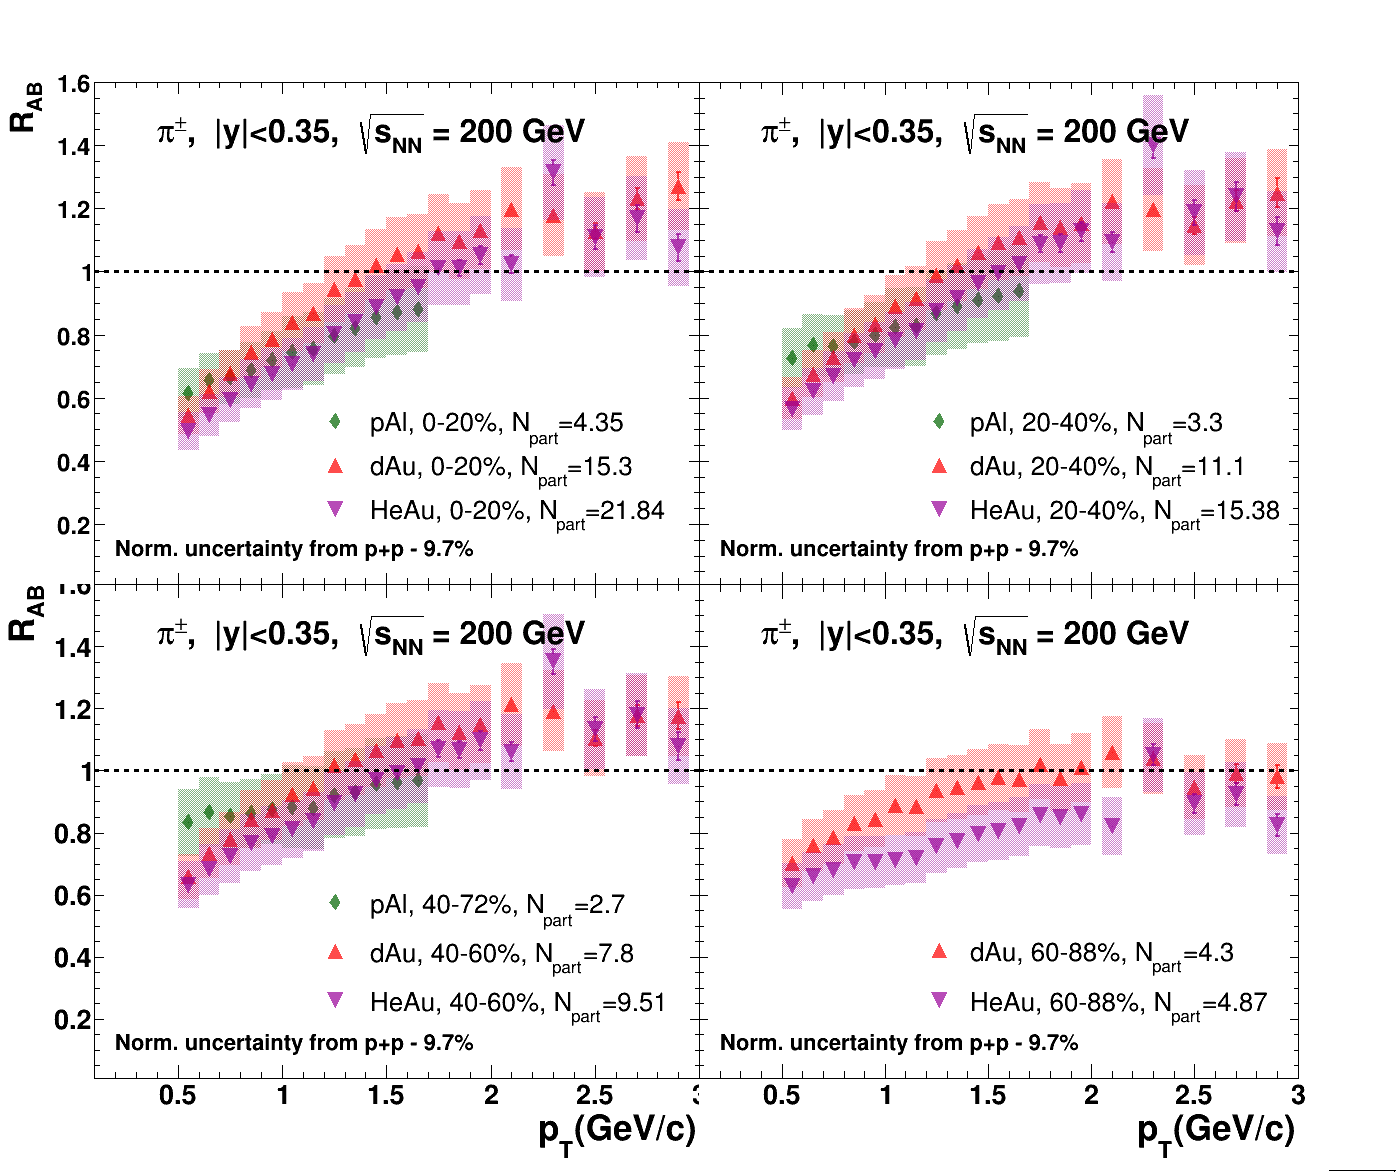
\includegraphics [width=0.7\linewidth]{Results/DrawAll_small_raa_1}
	\caption{Значения \rab \ измеренные для \pipm \ в различных центральностях столкновений \pal, \heau, $d$+Au.} 
	\label{img:Res_piRab_small}
\end{figure}

\begin{figure}[] 
	\centerfloat
	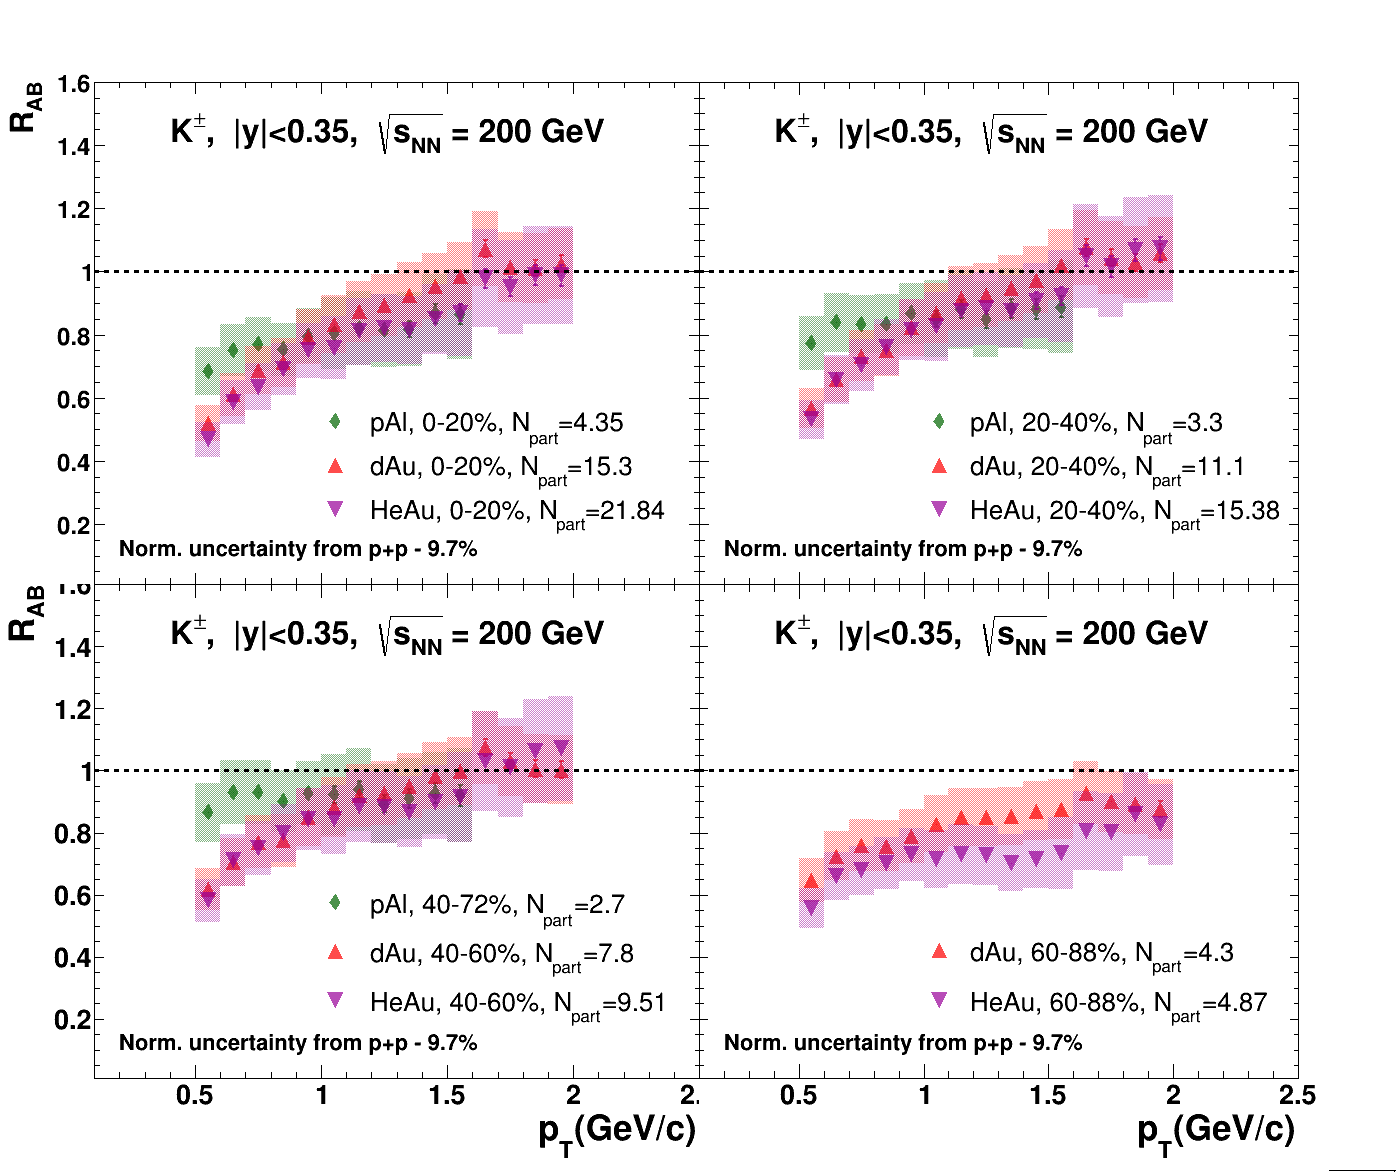
\includegraphics[width=0.7\linewidth]{Results/DrawAll_small_raa_2}
	\caption{Значения \rab \ измеренные для \Kpm \ в различных центральностях столкновений \pal, \heau, $d+Au$.} 
	\label{img:Res_KRab_small}
\end{figure}

\begin{figure}[] 
	\centerfloat
	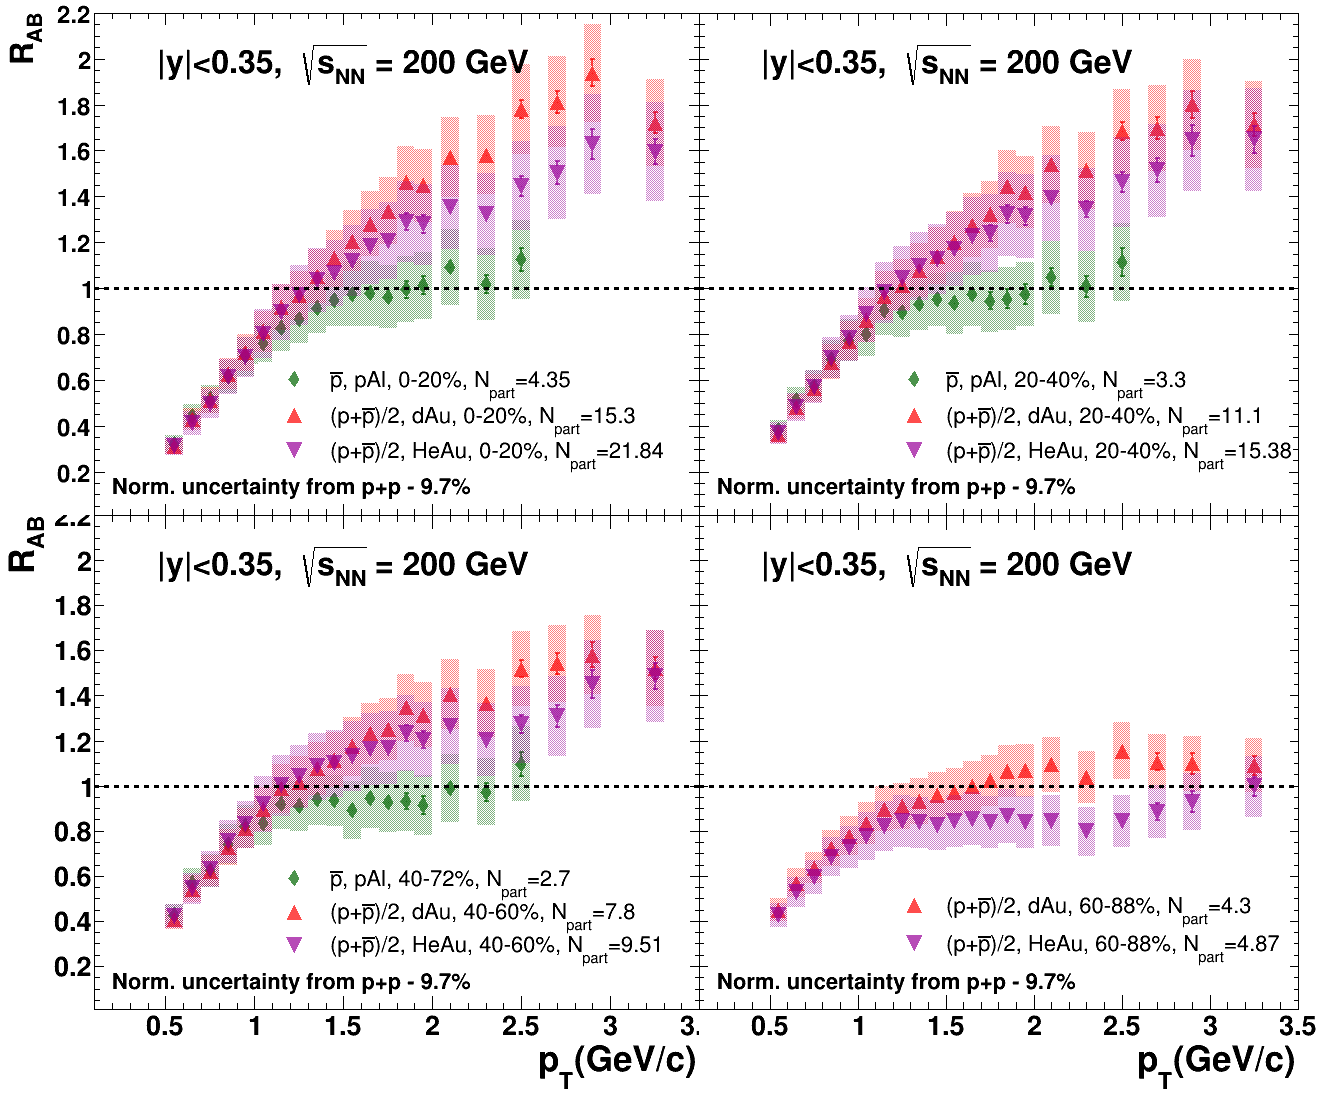
\includegraphics[width=0.7\linewidth]{Results/DrawAll_small_raa_3}
	\caption{Значения \rab \ измеренные для \aprot \ в различных центральностях столкновений \pal, и значения \rab, измеренные для \prots \ в различных центральностях \heau, $d+Au$ столкновений.} 
	\label{img:Res_pRab_small}
\end{figure}

На рис.\ref{img:Res_piRab_large}-\ref{img:Res_pRab_large} представлено сравнение значений \rab, измеренных для  \pipm, \Kpm-мезонов и \prots \ в \cuau \ и \auau \ столкновениях при энергии \sqsn=200 ГэВ, а также в \uu \ столкновениях при энергии \sqsn=193 ГэВ. Значения \rab, измеренные для заряженных адронов в различных системах, но при схожих значениях количества нуклонов-участников (\Npart), совпадают в пределах систематических неопределенностей. Данный результат может означать, что рождение заряженных адронов зависит от размера области перекрытия сталкивающихся ядер, но не зависит от ее формы.

На рис.\ref{img:Res_piRab_small}-\ref{img:Res_pRab_small} представлено сравнение значений \rab, измеренных для  \pipm, \Kpm-мезонов и \aprot \ в \pal \ столкновениях, и значений \rab, измеренных для \pipm, \Kpm-мезонов и \prots \ в \dau \ и \heau \ столкновениях при энергии \sqsn=200 ГэВ. Значения \rab, измеренные для \pipm, \Kpm-мезонов в различных системах, но при схожих значениях \Npart, совпадают в пределах погрешностей. Значения \rab, измеренные для \aprot \ в \pal \ столкновениях, близки к единице и меньше значений \rab, измеренных для \prots \ в \heau \ и \dau \ столкновениях. Также важно отметить, что зависимость значений \rab \ от \pt, измеренных для \pipm \ и \Kpm-мезонов в \pal \ столкновениях, имеет меньший наклон, чем наклон зависимостей значений \rab \ от \pt, измеренных для \pipm, \Kpm-мезонов в \dau \ и \heau \ столкновениях. 

\subsubsection{Сравнение факторов ядерной модификации легких адронов}
На рис. \ref{img:Res_HadronRab_large} показаны факторы ядерной модификации легких адронов в столкновениях тяжелых систем при энергии \sqsn=200 ГэВ. В центральных столкновениях значения протонных \rab \ превышают значения \rab, измеренные для мезонов, в промежуточном диапазоне \pt \ (1 ГэВ/c $< p_T <$ 3 ГэВ/с). В частности, значения \rab, измеренные для протонов, больше, чем значения \rab, измеренные для $\phi$-мезонов. Принимая во внимание, что масса $\phi$-мезона $m_{\phi}$=1.019 ГэВ$^{2}$ сравнима c массой протона, можно сделать вывод, что разница значений \rab \ не может быть объяснена зависимостью от массы частицы.  

%Увеличенный по сравнению с $p+p$ столкновениями выход протонов считается одним из характерных признаков образования КГП \cite{BaryonPuzzleVelkovska, BaryonPuzzle2002, BaryonPuzzleHeavy}.

Также в центральных столкновениях важно отметить совпадение значений \rab \ мезонов, содержащих странные кварки, таких как \Kstar, \phim \ и \Kpm. Значения \rab \ таких мезонов близки к единице. Значения \rab \ мезонов, которые не содержат странных кварков, таких как \pio \ и \pipm,  также совпадают между собой в промежуточном диапазоне \pt, однако имеют меньшие величины по сравнению с мезонами, содержащими странный кварк. Данная закономерность может указывать на эффект увеличения выхода странности, являющимся одним из основных признаков образования КГП \cite{Strangeness_QGP, StrangEnh, ThermalStrangeness}.

\begin{figure}[] 
	\centerfloat
	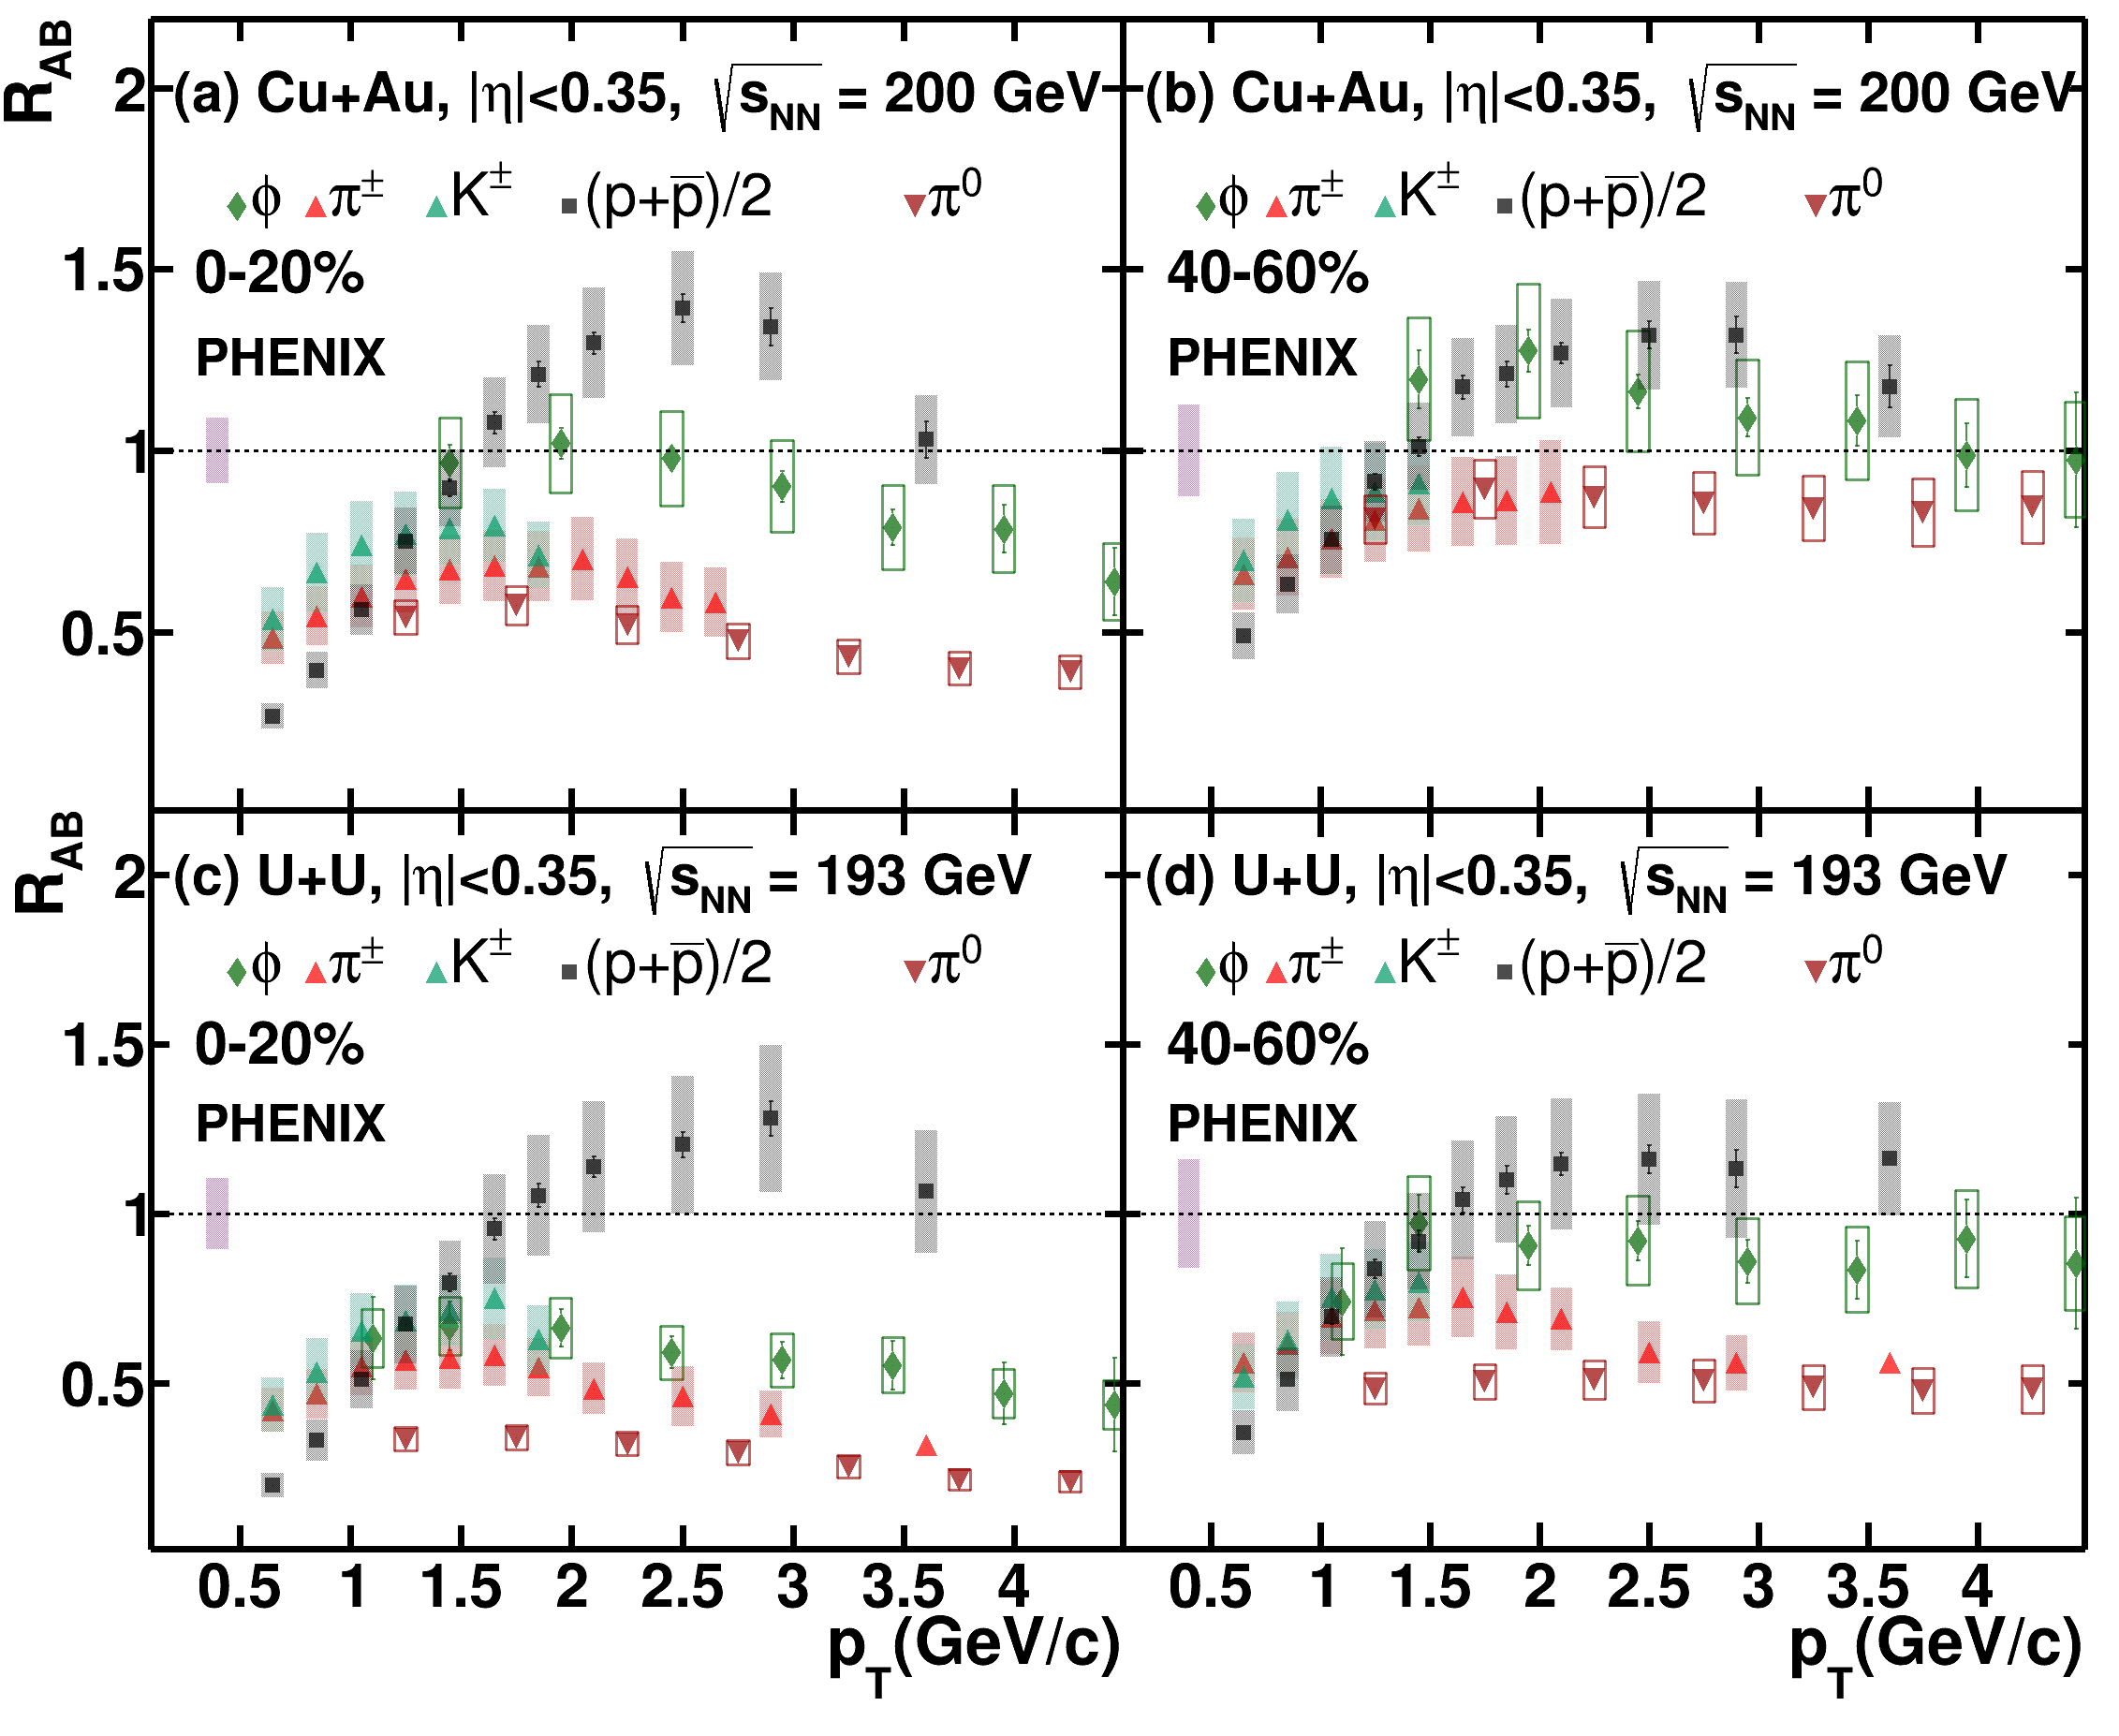
\includegraphics [width=0.7\linewidth]{Results/DrawMesons_large}
	\caption{Значения \rab  \ измеренные для легких адронов (\pipm, \pio, \Kstar, \Kpm, $\varphi$, \prots) в центральных и периферических столкновениях \cuau, \auau, \uu.} 
	\label{img:Res_HadronRab_large}
\end{figure}

На рис. \ref{img:Res_HadronRab_small} представлены значения \rab, измеренные для различных легких адронов (\pipm, \pio, \Kstar, \Kpm, $\varphi$, \prots) в легких системах столкновений (\pal \ и \heau).
Значения \rab \ всех рассматриваемых мезонов совпадают в пределах погрешностей как в центральных, так и в периферийных столкновениях \pal \ и \heau. В частности, значения \rab, измеренные для мезонов, содержащих странный кварк (\phim, \Kpm, \Kstar) совпадают в пределах систематических неопределенностей со значениями \rab, измеренными для мезонов, не содержащих странный кварк (\pipm, \pio). Таким образом в столкновениях \pal \ и \heau \ не наблюдается увеличенный выход странности. 
Увеличенный по сравнению с $p+p$ столкновениями (\rab>1) выход протонов наблюдается только в центральных столкновениях \heau. В  \pal столкновениях и периферийных столкновениях \heau \ значения \rab \ протонов совпадают со значениями \rab \ мезонов в пределах систематических неопределенностей.  

\begin{figure}[] 
	\centerfloat
	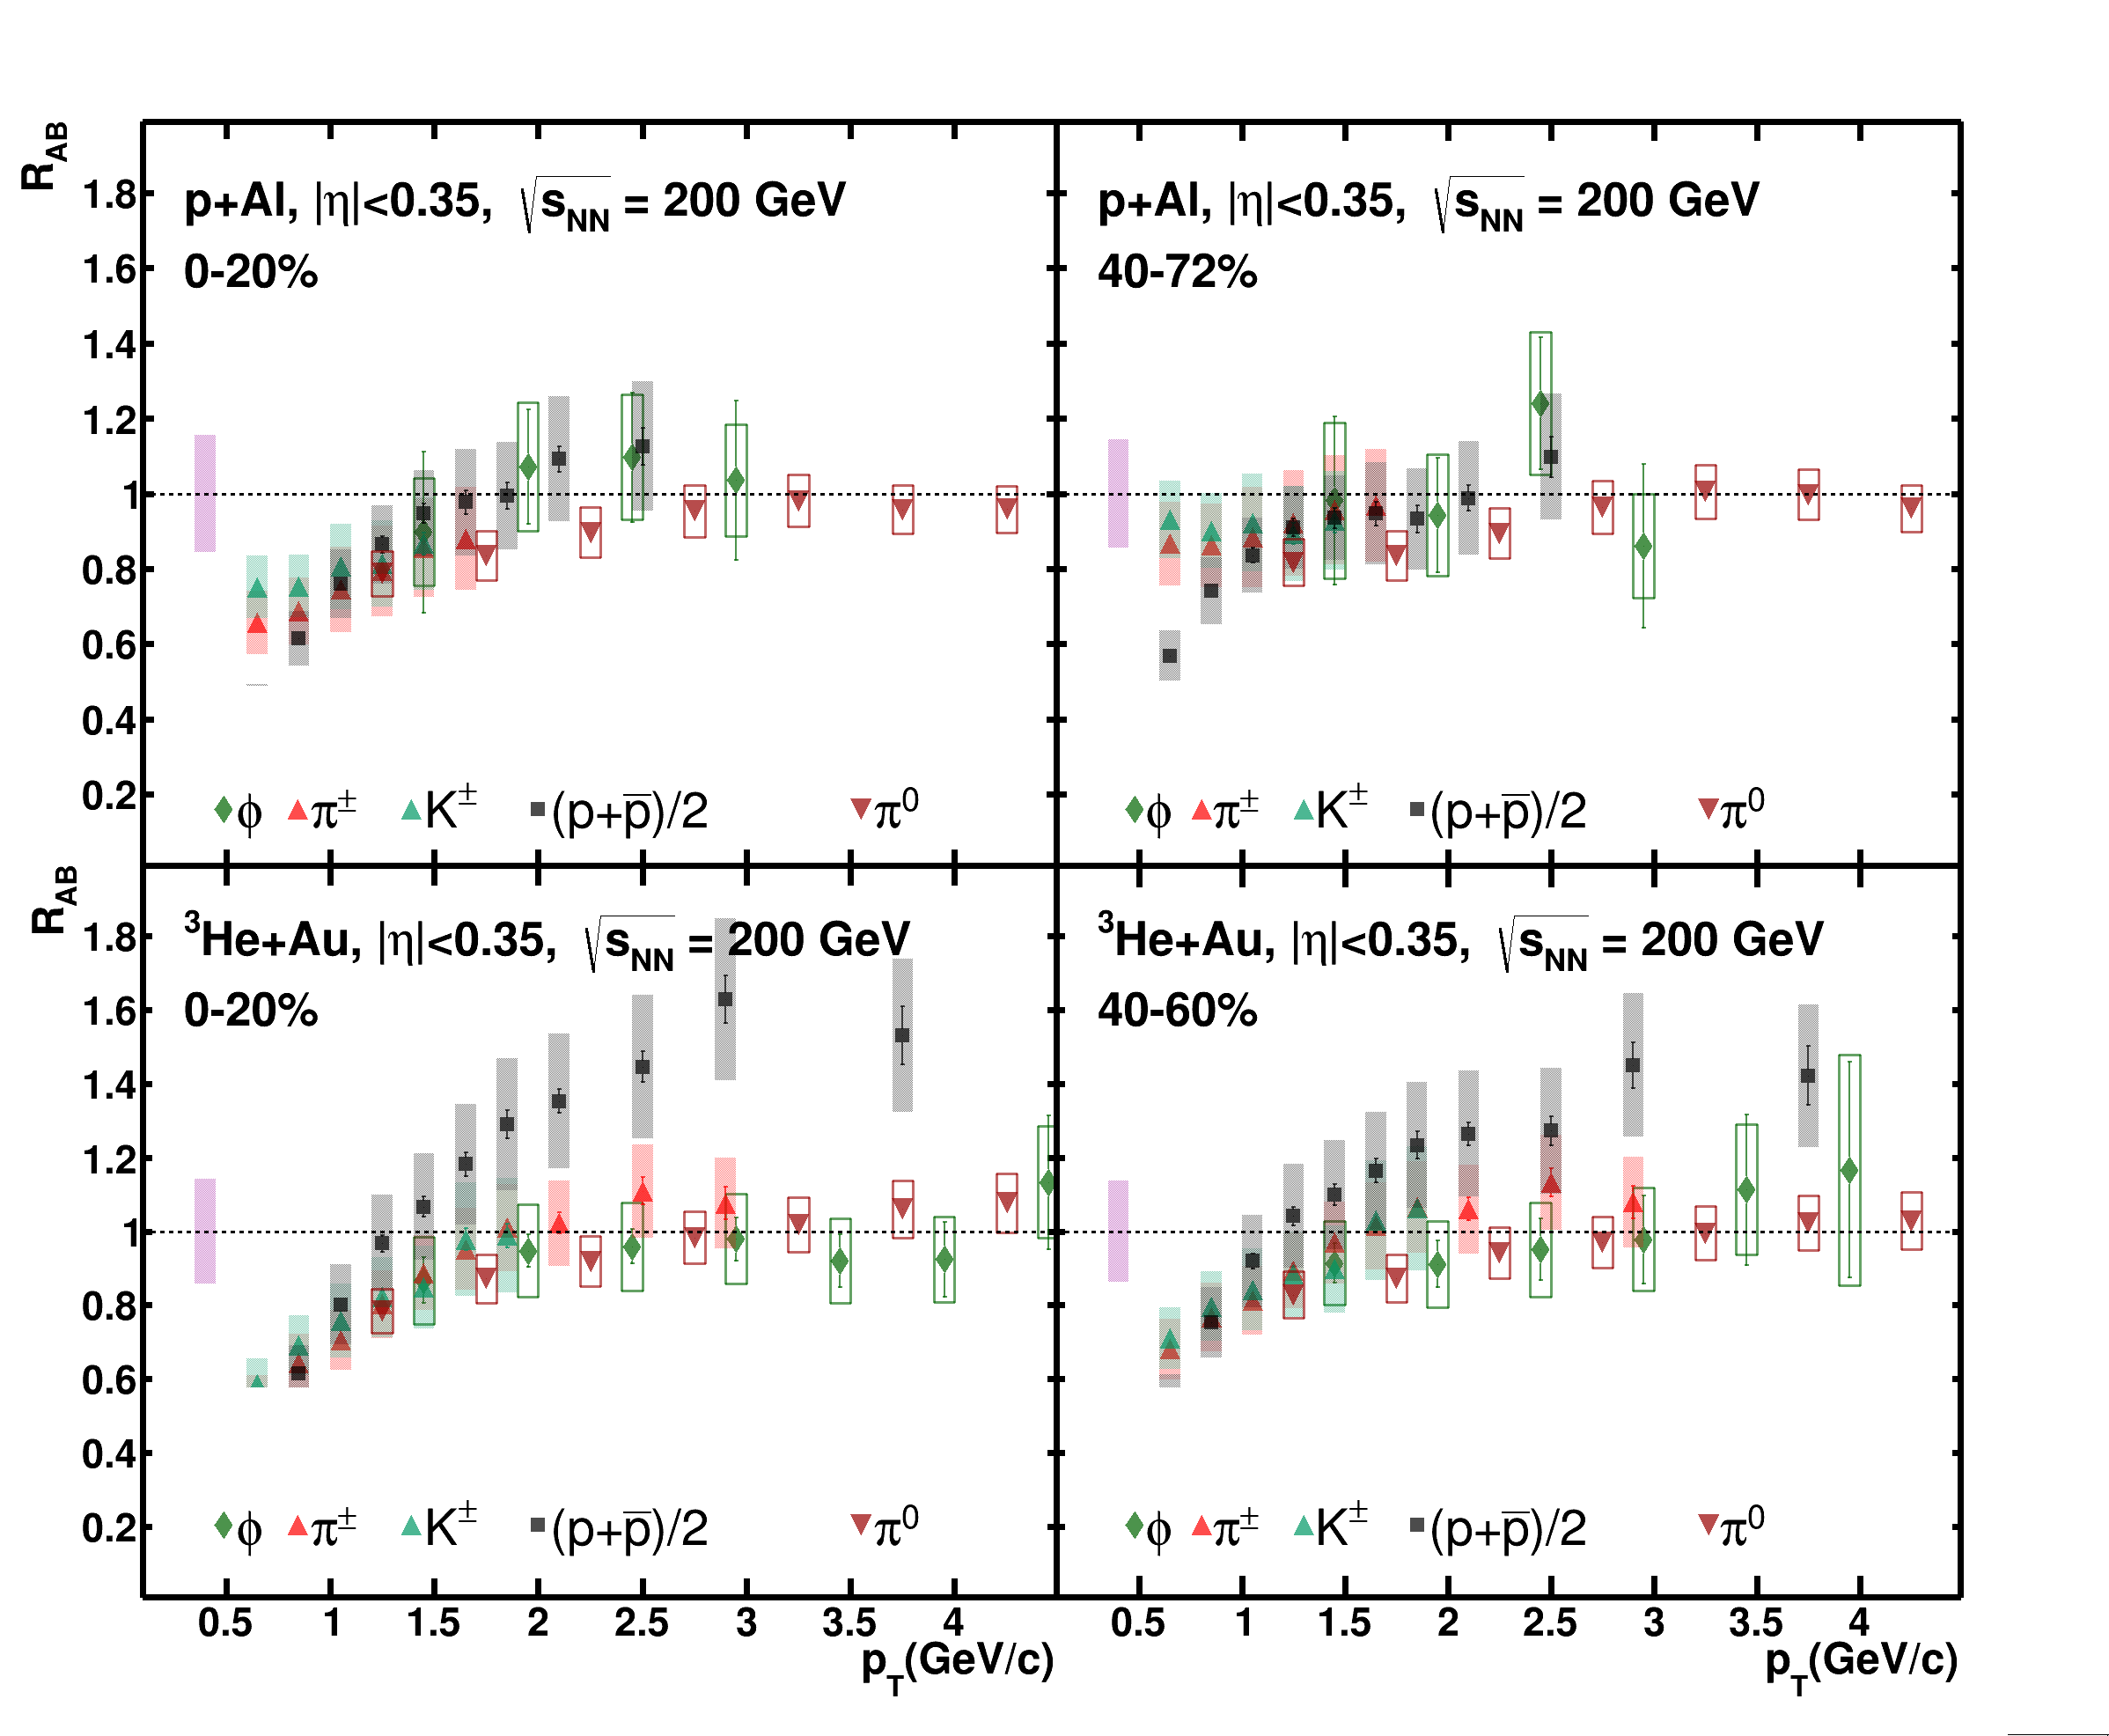
\includegraphics [width=0.7\linewidth]{Results/DrawMesons_small}
	\caption{Значения \rab \ измеренные для легких адронов (\pipm,\pio,\Kstar,\Kpm,\phim,\prots) в центральных и периферических столкновениях \pal, \dau, \heau} 
	\label{img:Res_HadronRab_small}
\end{figure}


\section{Отношения выходов \ratppi~ и \ratKpi}
С целью более детального изучения различий в процессах образования протонов и мезонов были вычислены следующие отношения инвариантных спектров частиц: $p/\pi^{+}$, $\bar{p}/\pi^{-}$, $K^{+}/\pi^{+}$, $K^{-}/\pi^{-}$.


%\begin{equation}
	%\label{eq:ratios}
	%p/\pi = \frac{(d^2 N_p)/(dp_T dy)}{(d^2 N_{\pi})(d p_T dy)}    
%\end{equation}

\begin{figure}[] 
	\centerfloat
	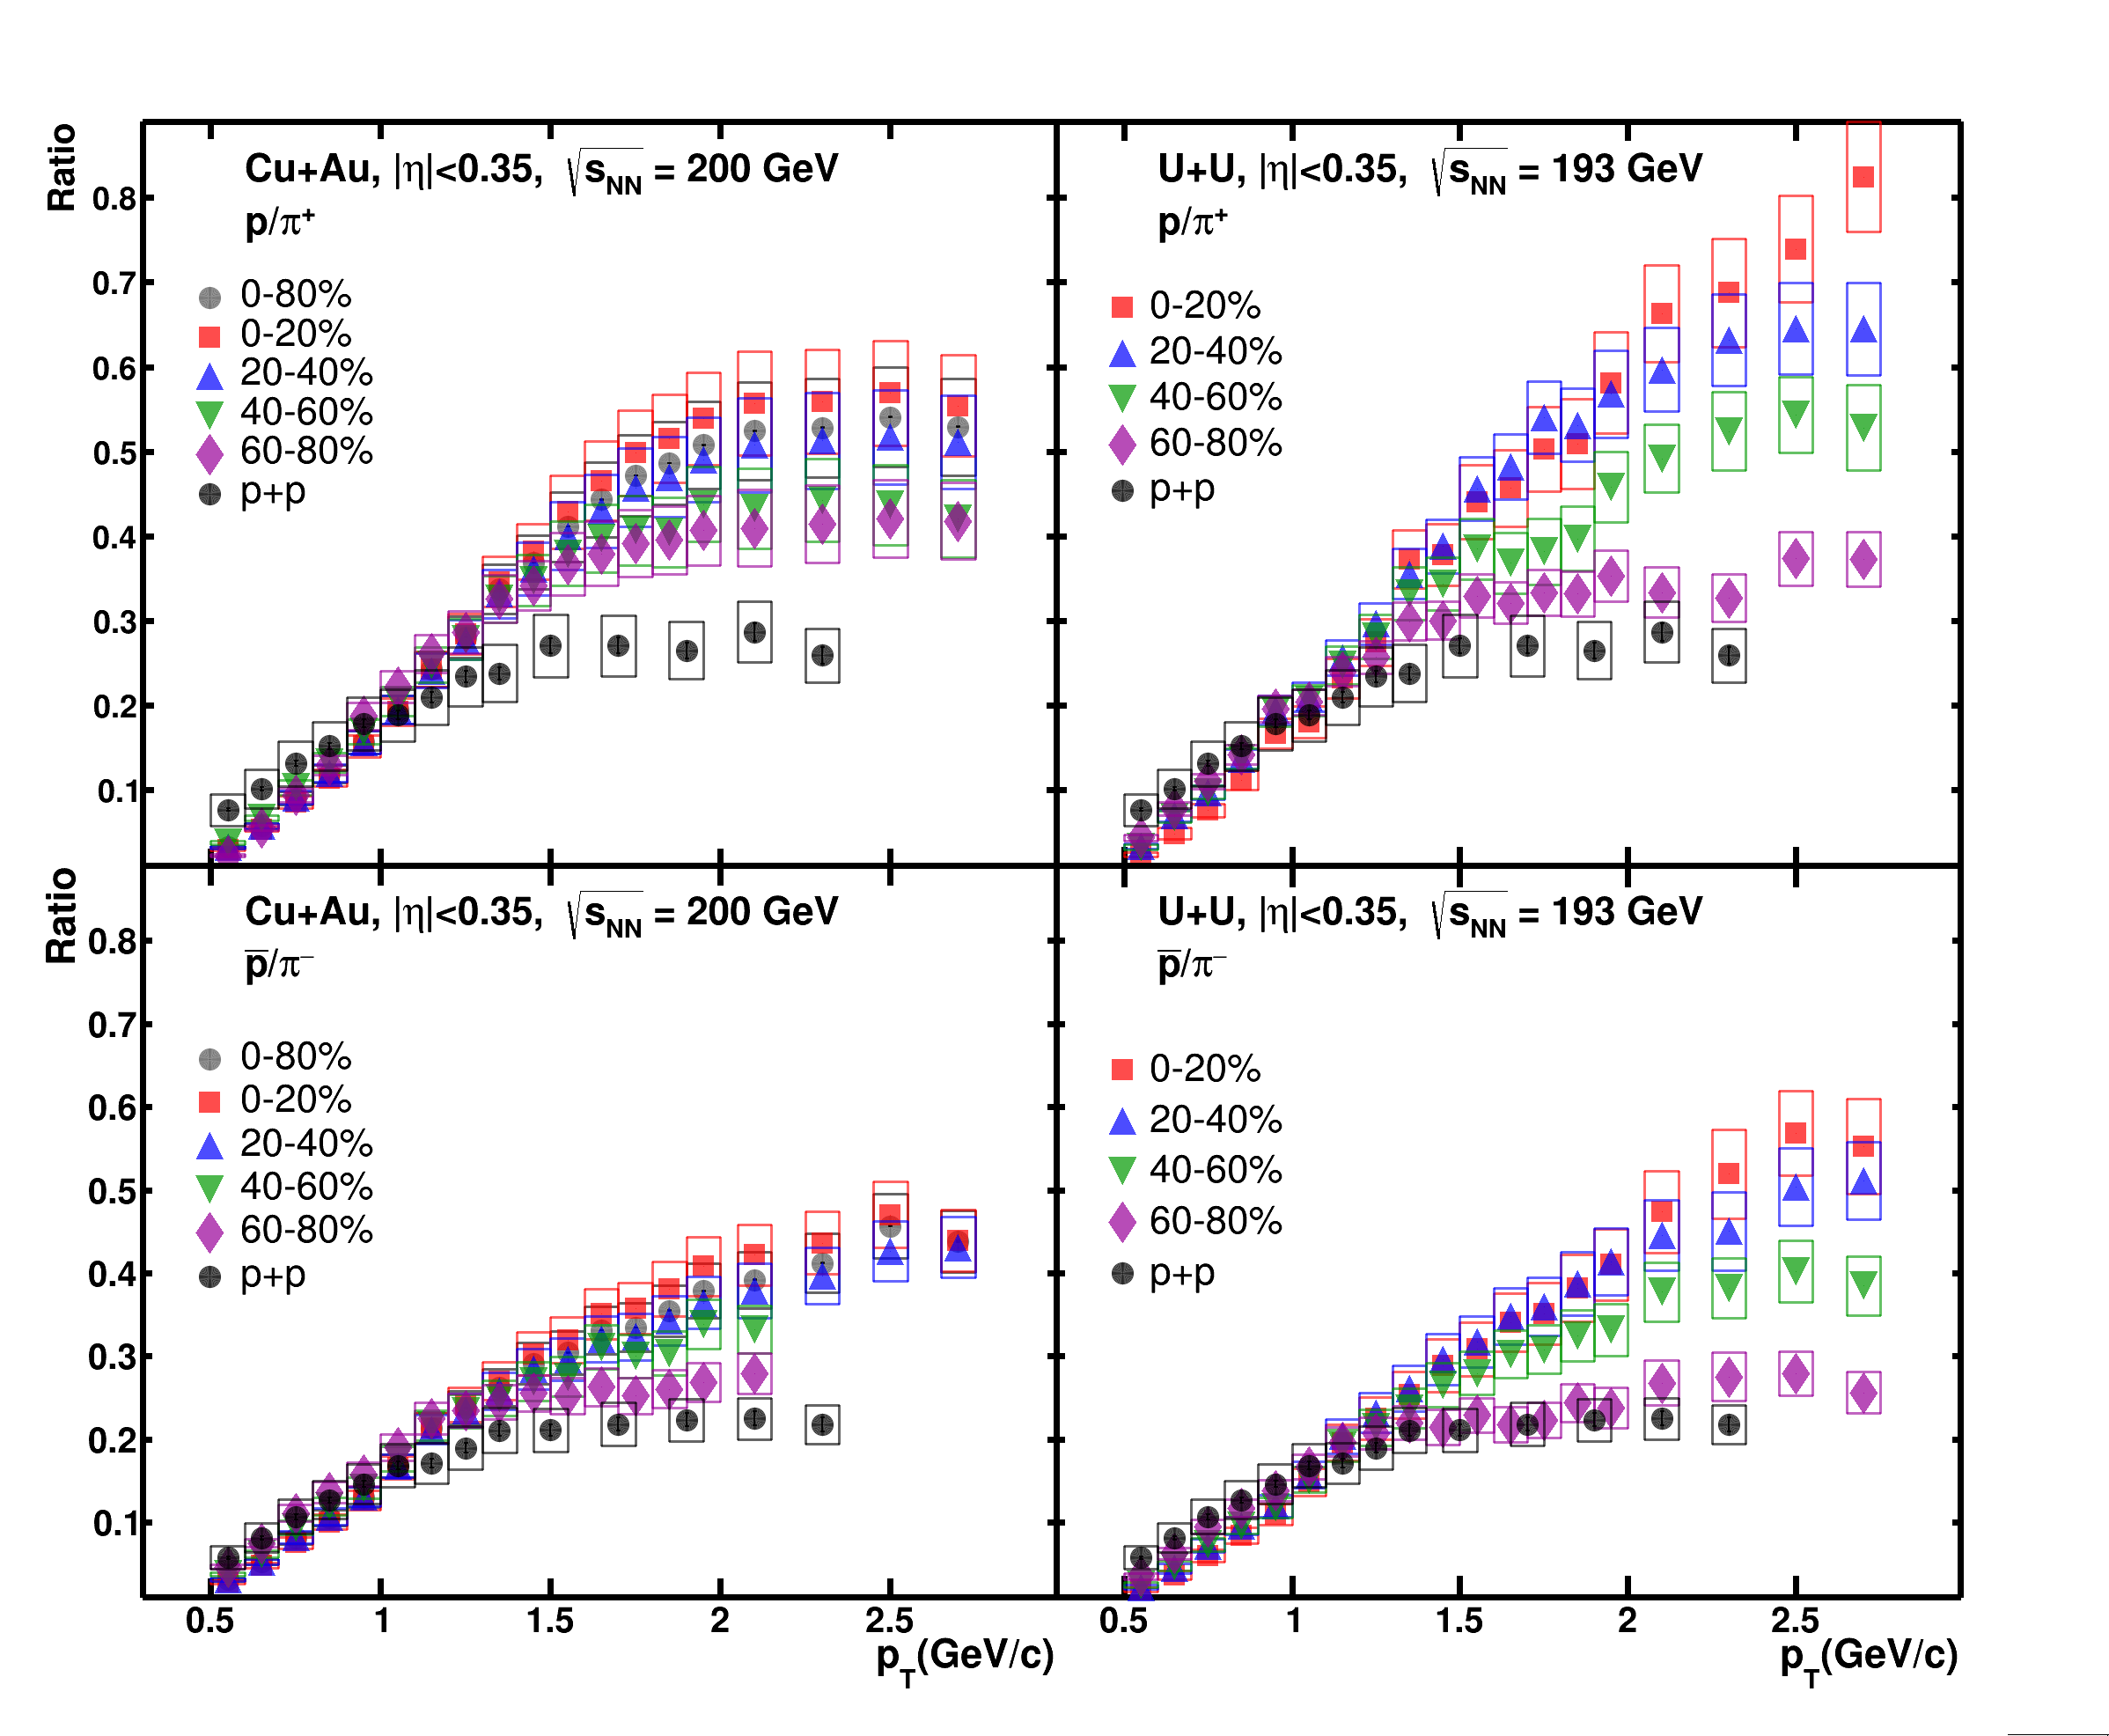
\includegraphics [width=0.7\linewidth]{Results/InOneCanvasHmy_large_p2pi}
	\caption{Значения отношений \ratppi \ в различных центральностях \cuau \ и \uu \ столкновений.} 
	\label{img:Res_p2pi_large}
	
\end{figure}

\begin{figure}[] 
	
	\centerfloat
	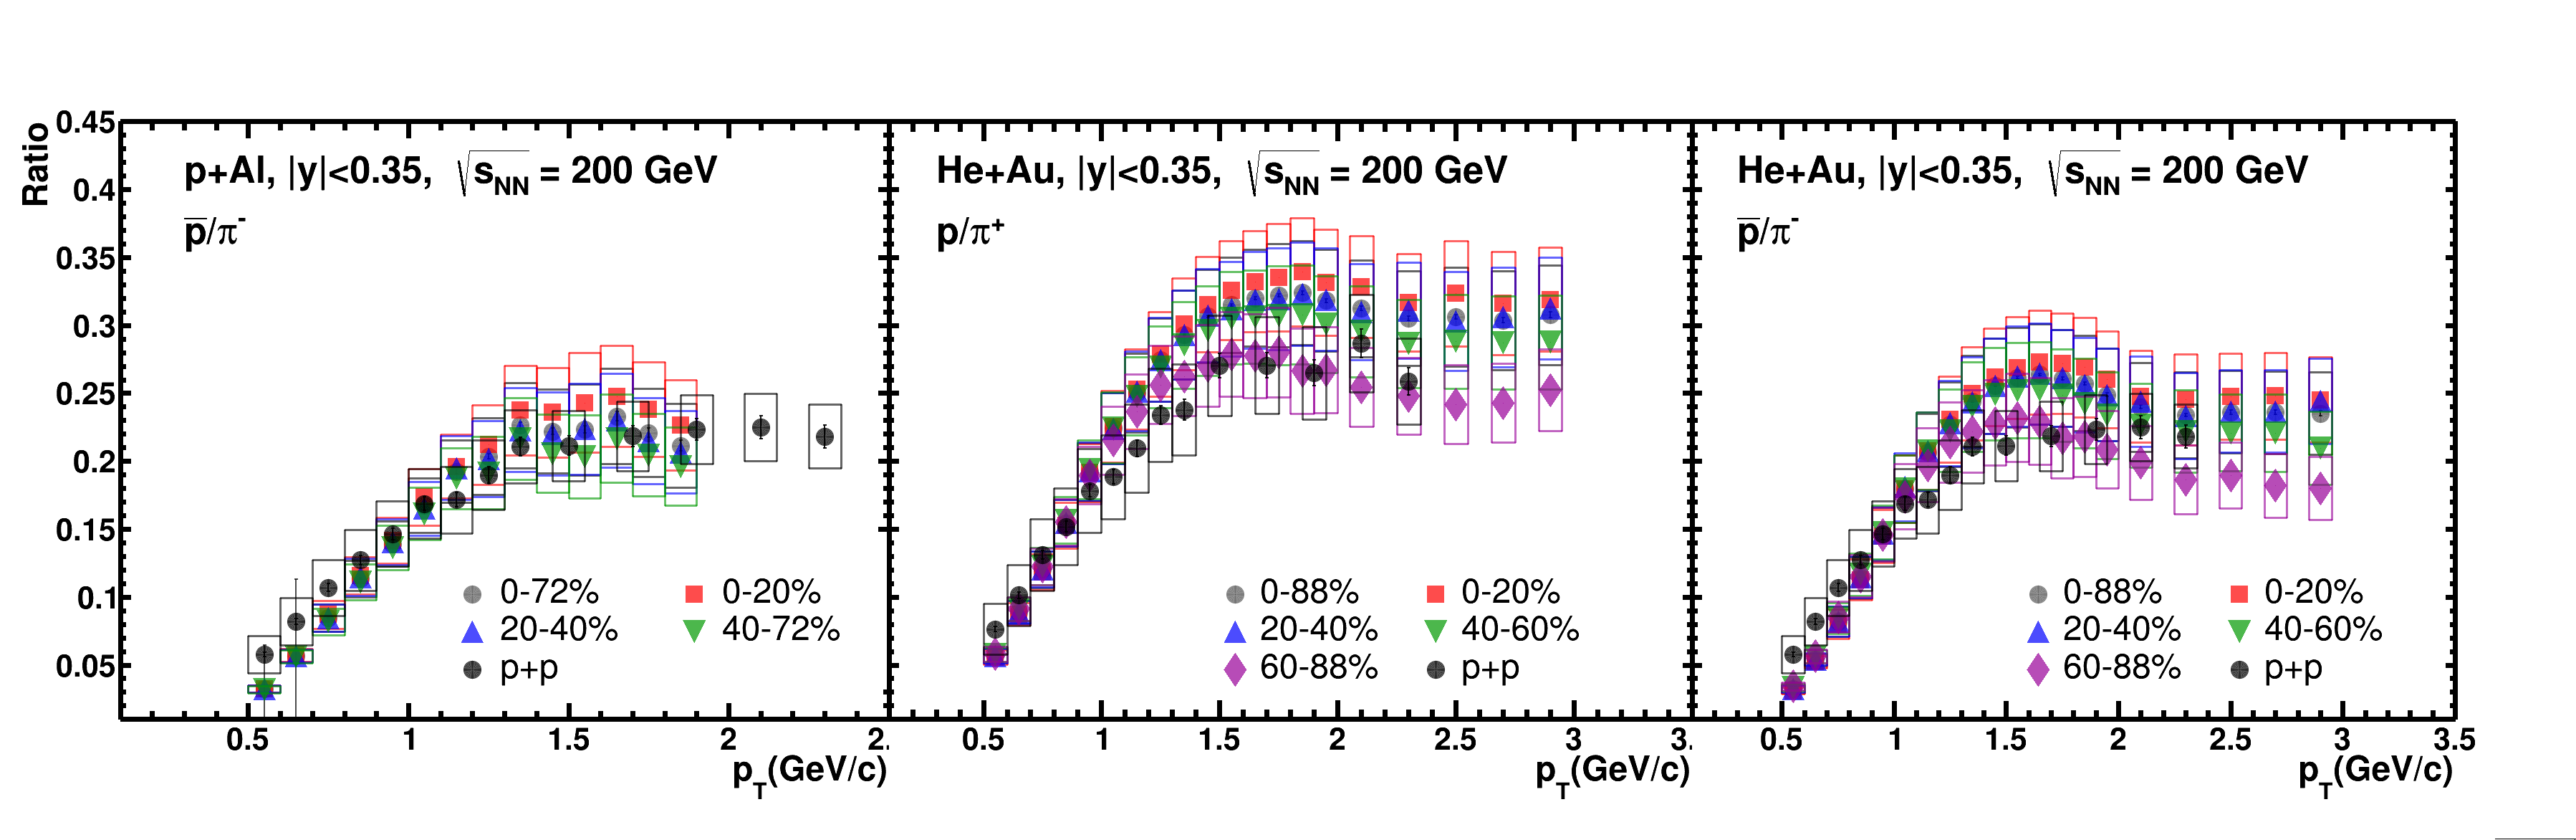
\includegraphics [width=1\linewidth]{Results/InOneCanvasHmy_small_p2pi}
	\caption{Значения отношений \ratppi \ в различных центральностях $p$+Al и \heau \ столкновений.} 
	\label{img:Res_p2pi_small}
\end{figure}

На рисунке \ref{img:Res_p2pi_large} представлено сравнение отношений \prot/\pip \ и \aprot/\pim \ в различных центральностях Cu+Au и U+U систем столкновений.
Величины отношений $p$/$\pi$, измеренные в Cu+Au и U+U столкновениях, достигают значения 0.8, что в $\sim2$ раза превосходит мксимальное значение $p$/$\pi$, измеренное в $p+p$ столкновениях. Также важно ометить, что значения \ratppi \ проявляют выраженную зависимость от центральности.
Увеличение значений \ratppi \ и из зависимость от центральности столкновения ранее были обнаружены в столкновениях Au+Au и интерпретированы в рамках рекомбинационной модели (см. раздел \ref{ch1/Recombination}) \cite{Recombination1, Recombination2}.

Отношения \ratppi, измеренные в различных классах событий по центральности в легких системах столкновений (\pal \ и \heau) представлены на рис \ref{img:Res_p2pi_small}. Зависимость отношений \ratppi \ от центральности, ярко выраженная в тяжелых системах столкновений, в столкновениях \pal \ не наблюдается. В столкновениях \heau \ отношения \ratppi \ проявляют слабую зависимость от центральности, которая однако незначима в связи с большими систематическими неопределенностями. 

\begin{figure}[] 
	\centerfloat
	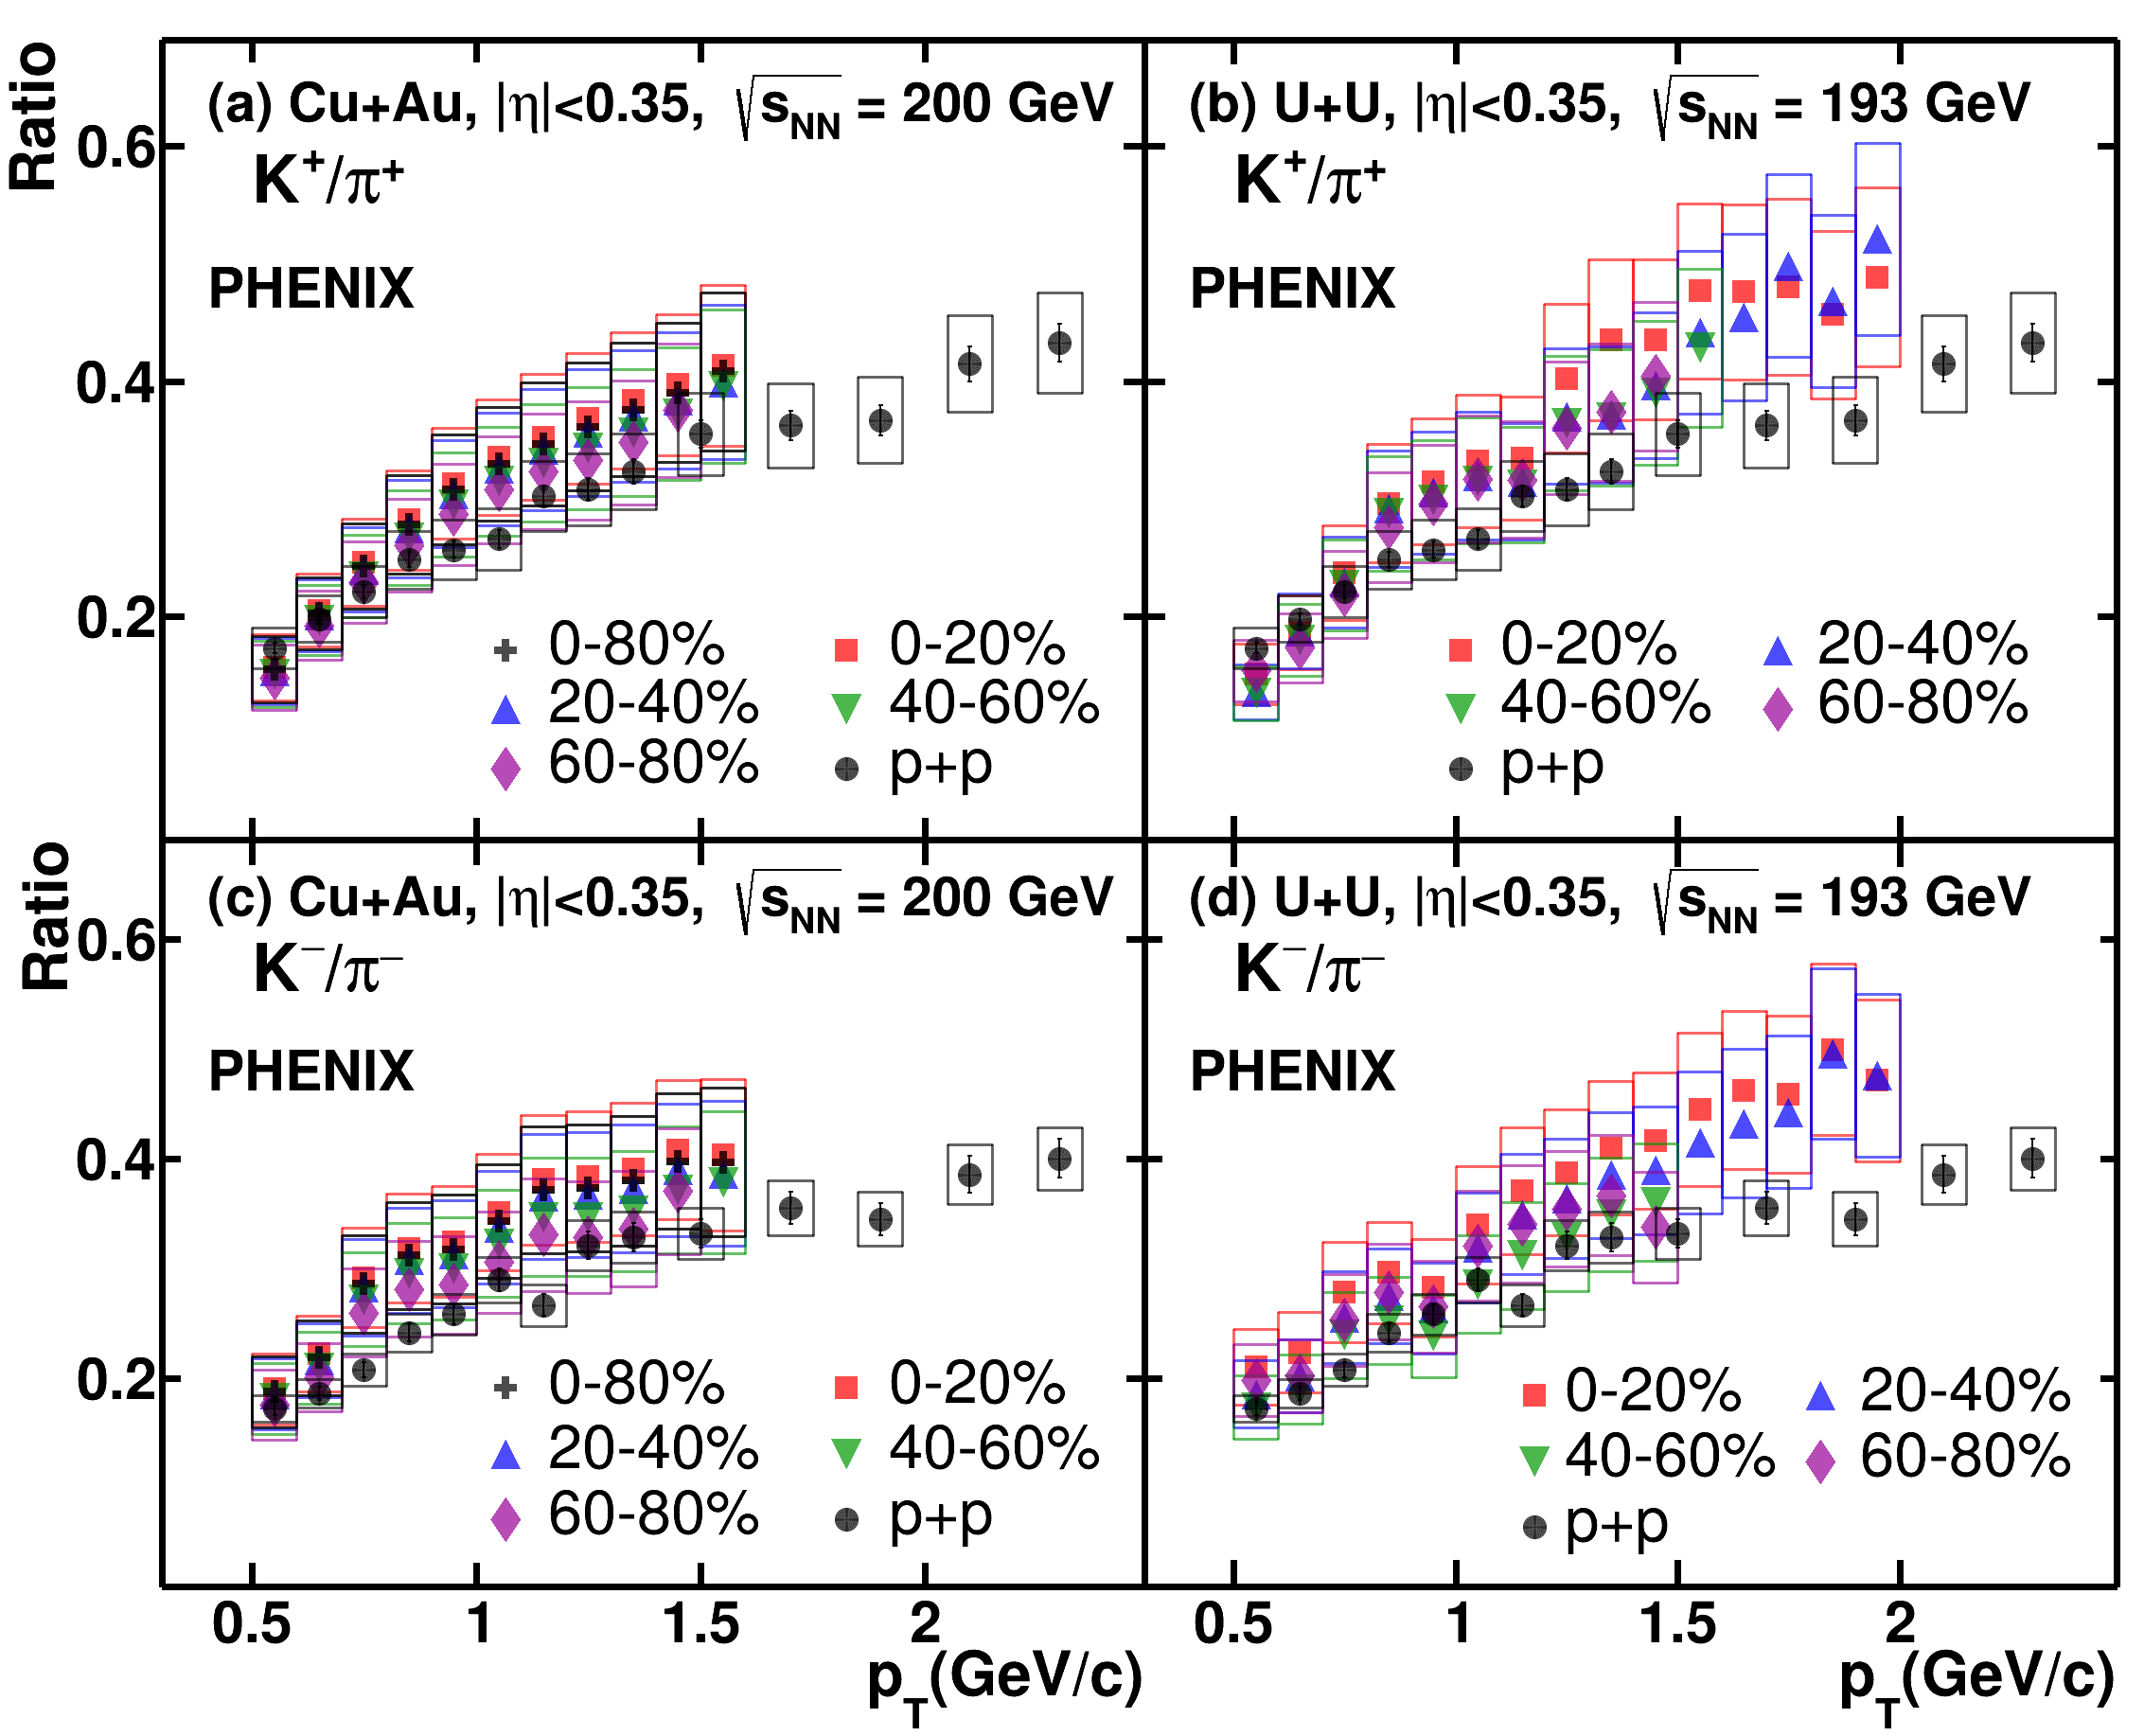
\includegraphics [width=0.7\linewidth]{Results/InOneCanvasHmy_large_K2pi}
	\caption{Значения отношений \ratKpi \ в различных центральностях \cuau, \auau, \uu \ столкновений.} 
	\label{img:Res_K2pi_large}
\end{figure}

\begin{figure}[] 
	\centerfloat
	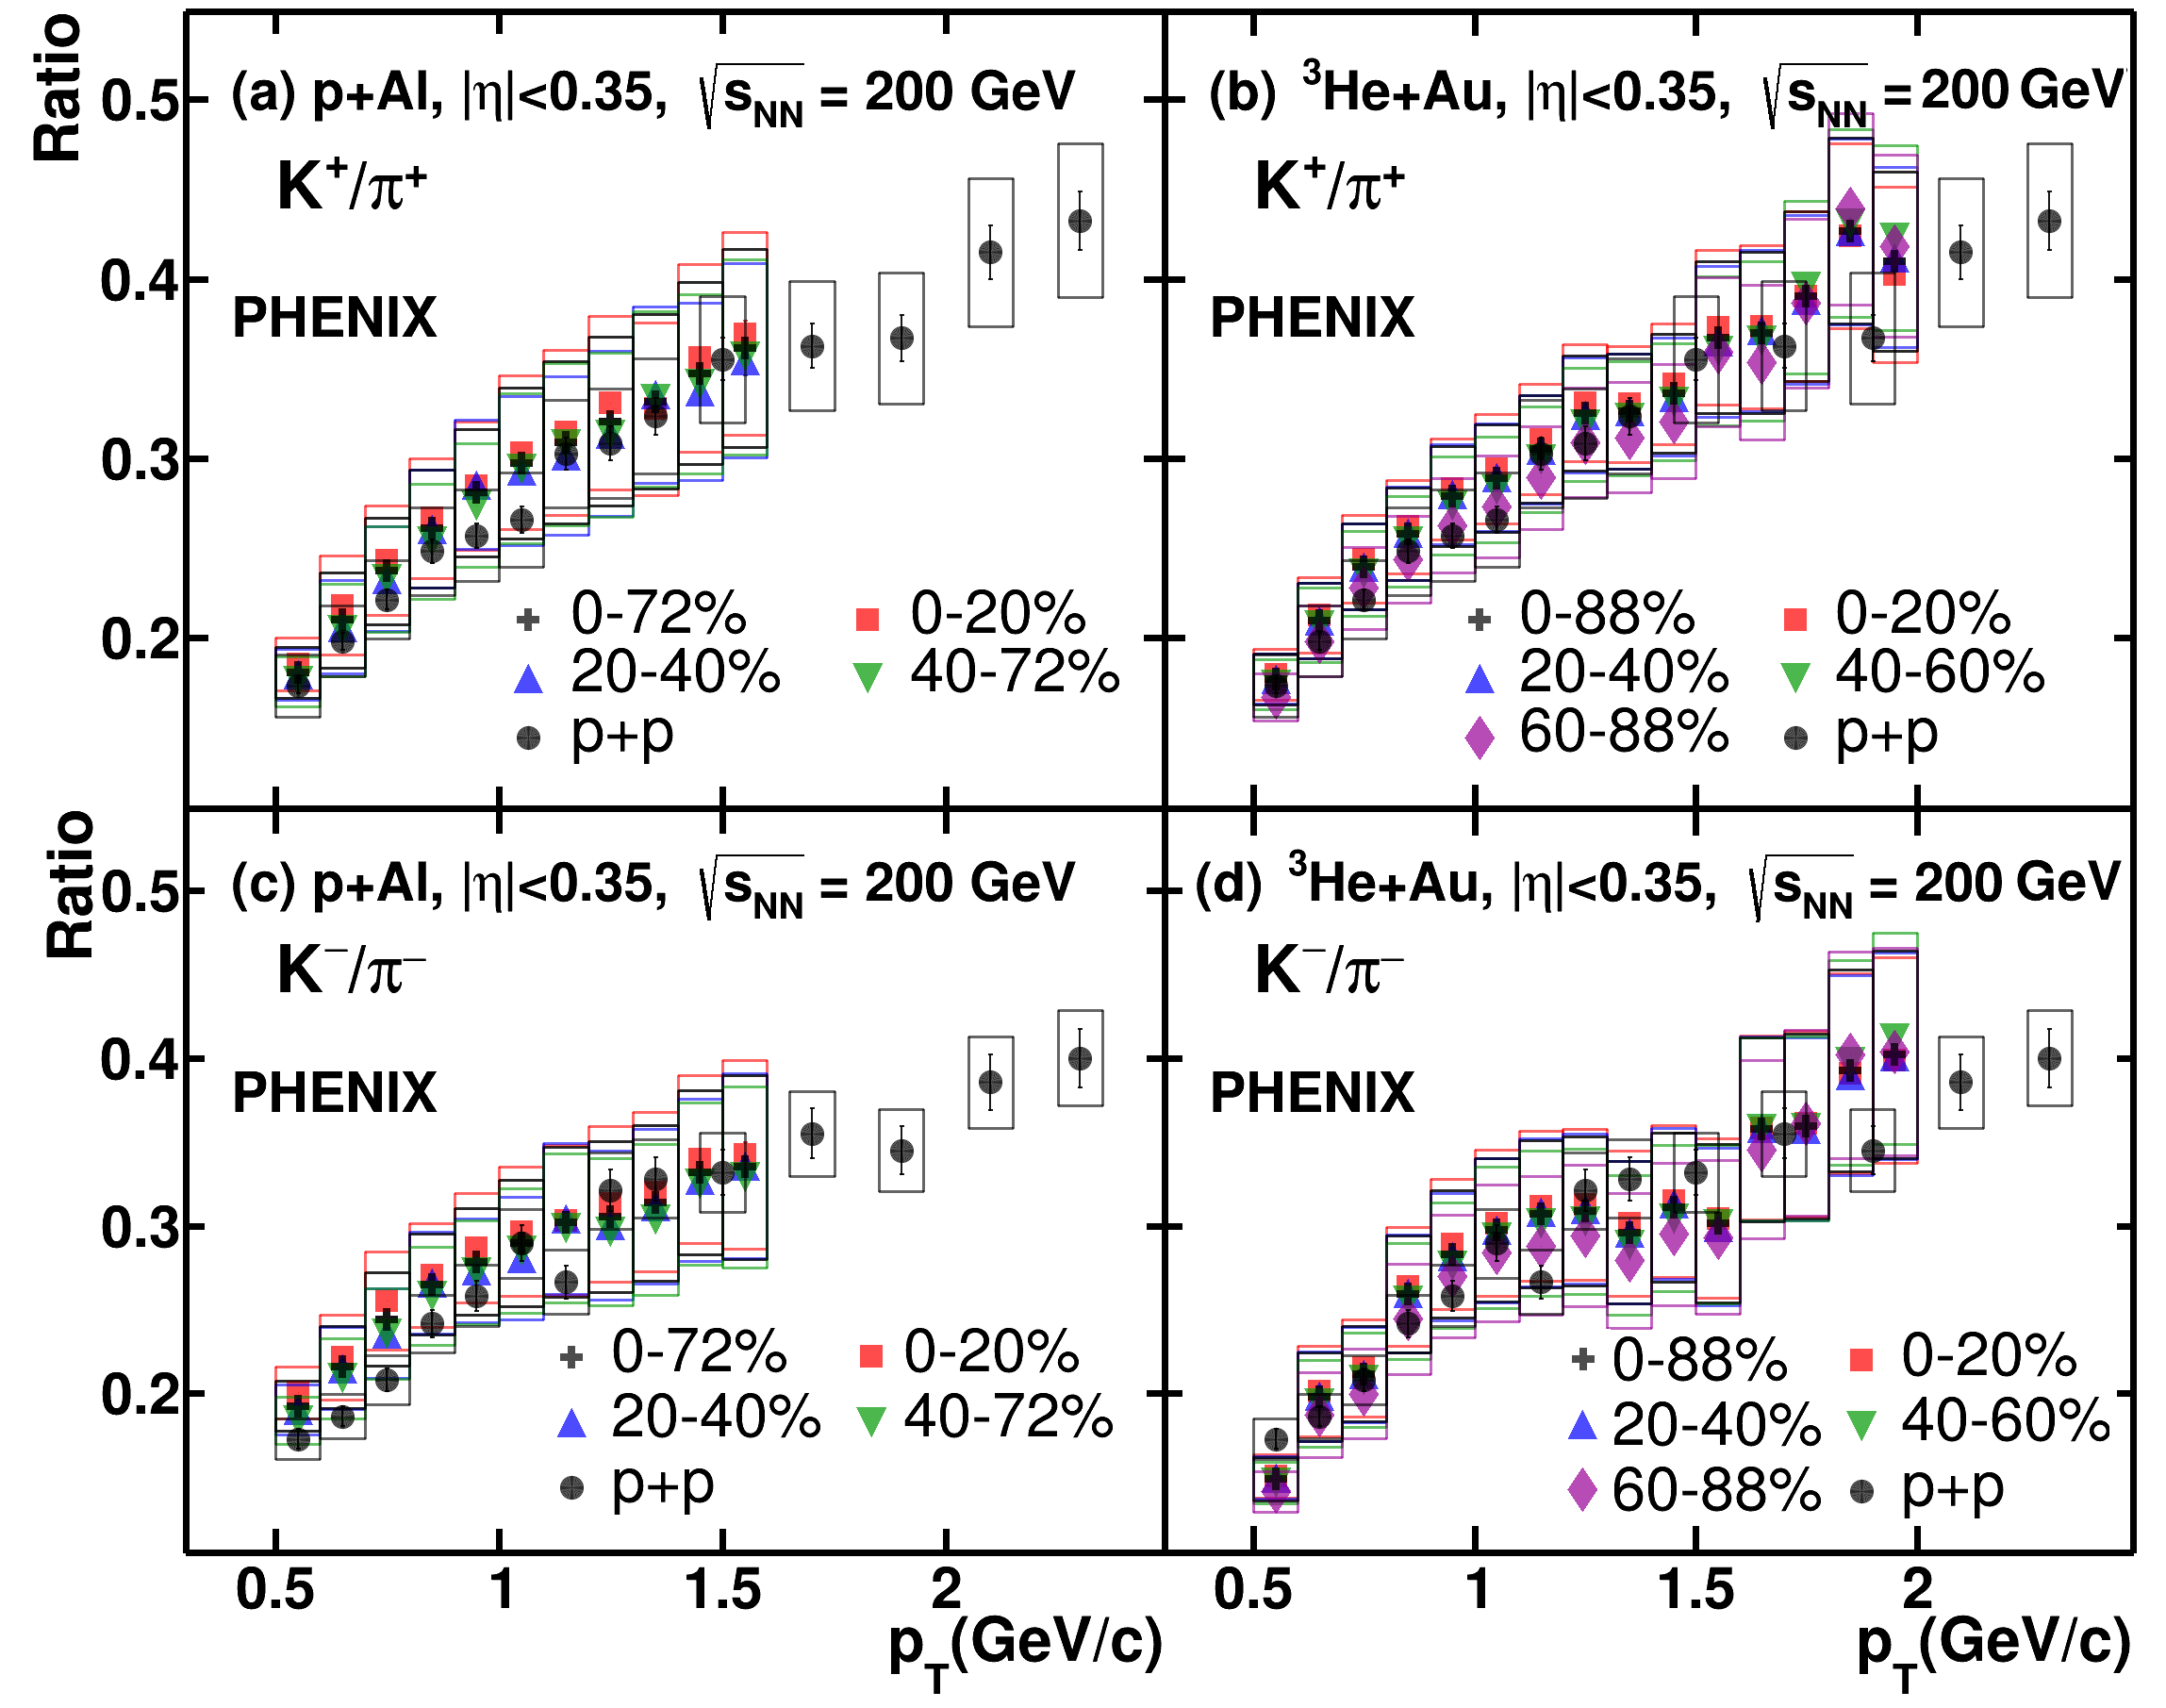
\includegraphics [width=0.7\linewidth]{Results/InOneCanvasHmy_small_K2pi}
	\caption{Значения отношений \ratKpi \ в различных центральностях \pal, \dau, \heau столкновений.} 
	\label{img:Res_K2pi_small}
\end{figure}
Также выли исследованы отношения инвариантных спектров, измеренные для двух типов мезонов: содержащего странный кварк $K$-мезона и $\pi$-мезона, состоящего только из $u$ и $d$ кварков (\ratKpi).
Во всех рассматриваемых системах столкновений значения отношений \ratKpi \ проявляют слабую зависимость от центральности центральности и по величине совпадают с результатами, полученными в $p+p$ столкновених  (рис. \ref{img:Res_K2pi_large}, \ref{img:Res_K2pi_small}). 
%Намек на зависимость величин $k/\pi$ от центральности, наблюдаемый в тяжелых системах столкновений является проявлением эффекта увеличенного выхода странности.
